\chapter{自旋液体和格点规范场}\label{chap:spin-liquid}

分数量子霍尔效应出现之后显然不出意外地引起了巨大的反响。很自然的想法是寻找更多具有拓扑序的系统,并且,通过研究“干净”一些的系统,或许可以分析出拓扑序的一些机制。
自旋液体是一类展现了拓扑序的自旋系统,它们可能对理解拓扑序中的概念有帮助,或者是有可能展现拓扑序的系统的演生理论。

大部分自旋系统(如\autoref{chap:magnetic}中展示的那些)在低温下都会落到铁磁序或反铁磁序中,因为零温时没有热涨落,而相互作用总是存在的,因此系统倾向于有序。
然而,如果零温时有特别强的量子涨落,可能系统基态中不存在这种类型的序,其中没有出现任何对称性自发破缺,无法定义序参量。
这样的自旋系统称为\concept{自旋液体},因为它们的基态是无序的,正如液体之于固体一样。
自旋液体的出现可能是因为在零温下由于一些阻挫(frustration, 即,让晶格取特定的形式使得反铁磁序无法形成)或者别的原因。
阻挫未必导致自旋液体,而也有自旋液体完全没有阻挫(比如Toric-code模型)。自旋液体如何能够形成实际上仍然是不太确定的。
需注意自旋液体中没有对称性自发破缺,但是这并不代表自旋液体中没有其它类型的序和相变,例如,它们完全可以有拓扑序。
因此,自旋液体是一个非常有趣的状态,其制备方法以及性质都很引人注意。

虽然自旋液体似乎可以归结在磁性材料的范畴内,强烈的量子涨落实际上意味着自旋液体中有一些一般的磁性材料不会有的丰富行为。
在真正的自旋液体中我们会观察到演生规范场和拓扑序——实际上,自旋液体是除了分数量子霍尔效应以外仅有的已知的在实验上有可能实现的拓扑序。
分数量子霍尔效应确定有拓扑序,而目前没有确定无疑是自旋液体的材料,其它的拓扑序模型都是人为构造的。

\begin{figure}
    \centering
    \tikzset{every picture/.style={line width=0.75pt}} %set default line width to 0.75pt        

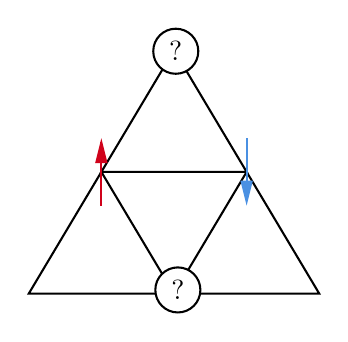
\begin{tikzpicture}[x=0.75pt,y=0.75pt,yscale=-1,xscale=1]
%uncomment if require: \path (0,300); %set diagram left start at 0, and has height of 300

%Shape: Triangle [id:dp3265971145624944] 
\draw   (225,126.33) -- (260,185) -- (190,185) -- cycle ;
%Shape: Triangle [id:dp457754747303309] 
\draw   (155,126.33) -- (190,185) -- (120,185) -- cycle ;
%Shape: Triangle [id:dp5282716496110524] 
\draw   (190,67.66) -- (225,126.33) -- (155,126.33) -- cycle ;
%Straight Lines [id:da7008008238341734] 
\draw [color={rgb, 255:red, 208; green, 2; blue, 27 }  ,draw opacity=1 ]   (155,142.56) -- (155,112.1) ;
\draw [shift={(155,110.1)}, rotate = 450] [fill={rgb, 255:red, 208; green, 2; blue, 27 }  ,fill opacity=1 ][line width=0.08]  [draw opacity=0] (12,-3) -- (0,0) -- (12,3) -- cycle    ;
%Straight Lines [id:da47122065737438956] 
\draw [color={rgb, 255:red, 74; green, 144; blue, 226 }  ,draw opacity=1 ]   (225,110.1) -- (225,140.56) ;
\draw [shift={(225,142.56)}, rotate = 270] [fill={rgb, 255:red, 74; green, 144; blue, 226 }  ,fill opacity=1 ][line width=0.08]  [draw opacity=0] (12,-3) -- (0,0) -- (12,3) -- cycle    ;
%Shape: Circle [id:dp2858034795038058] 
\draw  [fill={rgb, 255:red, 255; green, 255; blue, 255 }  ,fill opacity=1 ] (181,183.18) .. controls (181,177.19) and (185.86,172.33) .. (191.85,172.33) .. controls (197.85,172.33) and (202.71,177.19) .. (202.71,183.18) .. controls (202.71,189.18) and (197.85,194.04) .. (191.85,194.04) .. controls (185.86,194.04) and (181,189.18) .. (181,183.18) -- cycle ;

%Shape: Circle [id:dp48141040110301847] 
\draw  [fill={rgb, 255:red, 255; green, 255; blue, 255 }  ,fill opacity=1 ] (180,68.18) .. controls (180,62.19) and (184.86,57.33) .. (190.85,57.33) .. controls (196.85,57.33) and (201.71,62.19) .. (201.71,68.18) .. controls (201.71,74.18) and (196.85,79.04) .. (190.85,79.04) .. controls (184.86,79.04) and (180,74.18) .. (180,68.18) -- cycle ;


% Text Node
\draw (191.85,183.18) node   [align=left] {?};
% Text Node
\draw (190.85,68.18) node   [align=left] {?};


\end{tikzpicture}
    \caption{三角晶格上的阻挫:无法适当安排自旋方向让相邻自旋反向}
    \label{fig:triangular-frustration}
\end{figure}

\begin{info}{寻找自旋液体的尝试}{try-finding-spin-liquid}
    目前没有人找到确定无疑是自旋液体的材料。
    1973年,P.W.Anderson考虑了一个三角晶格上的反铁磁模型,来给反铁磁序的形成制造一些阻挫,因为三角晶格上显然无法形成反铁磁序(见\autoref{fig:triangular-frustration})。
    他猜测其基态为将晶格上最近邻自旋配对后将两个自旋自由度做分解
    \[
        \frac{1}{2} \otimes \frac{1}{2} = 0 \oplus 1,
    \]
    取所有可能的配对中的单态等权叠加的结果。这个状态称为\concept{RVB(Resonance Valence Bond)态}。
    如果实际上基态真的是RVB态,那么显然基态上没有形成任何磁性序,并且会有一些和磁性序上的“扰动”截然不同的激发(这些后文会详述)。
    事实证明这个说法是错误的:三角晶格上的海森堡模型的基态是一种特殊的铁磁态。虽然如此,自旋液体仍然是一个非常有趣的状态,因为,这可能是因为,对称性破缺不能发生。
    一些有机盐被认为有可能产生自旋液体,因为对它们做AMR实验观察不到任何磁性序,但始终没有定论;不少这种候选的自旋液体都被其它实验证实并非自旋液体了。
\end{info}

\section{各向同性海森堡模型演生出的自旋液体}

各向同性海森堡模型是
\begin{equation}
    H = J \sum_{\pair{\vb*{i}, \vb*{j}}} \vb*{S}_{\vb*{i}} \cdot \vb*{S}_{\vb*{j}}.
    \label{eq:heisenberg-model-spin-liquid}
\end{equation}
我们没有指定晶格是什么;本节将假定此模型在某个晶格上能够形成自旋液体,并且将处理自旋液体的标准手法作用于其上。

\subsection{三角晶格上的RVB态及其附近的低能激发}

\begin{back}{部分子构造}{parton-spin}
    \concept{部分子方法}是指将一个自旋自由度写成一些费米子或是玻色子自由度(即所谓\concept{部分子})的组合,自旋算符是两个费米子或是玻色子产生湮灭算符的乘积,然后施加适当的约束来保证拆分后的物理和拆分前相同。
    这相当于说,我们使用一个费米子系统或是玻色子系统实现了一个自旋系统。
    这种方法有时也称为\concept{投影构造}。
    这样做的好处在于,如果由此得到的费米子或玻色子理论中相互作用没有强到让这些费米子和玻色子又凝聚成对,那么实际上,这意味着自旋系统演生出了类似于费米子和玻色子的激发,即拆分得到的部分子正是自旋系统的低能自由度。

    只要算符的代数关系不变,并且将部分子系统的希尔伯特空间固定为每个格点上只有一个部分子的那部分,不同的拆分方式不会改变物理。
    对自旋系统,我们手动给不同格点上的自旋算符贴上位置标签,而对费米子/玻色子系统,坐标标签是粒子产生算符自带的参数,因此表面上看起来,拆分之后得到的费米子/玻色子系统的希尔伯特空间由于对称化/反对称化的要求而受到限制,似乎部分子系统的希尔伯特空间要比自旋系统的希尔伯特空间小,但是实际上两者是同构的:自旋系统的希尔伯特空间的基形如
    \[
        \ket{\sigma_1, \sigma_2, \ldots, \sigma_n}
    \]
    而部分子系统的希尔伯特空间的基形如
    \[
        {c}^\dagger_{1 \sigma_1} {c}^\dagger_{2 \sigma_2} \cdots {c}^\dagger_{n \sigma_n} \ket{0},
    \]
    后者中交换$1, 2$等空间标签,态矢量不变或者反号,所以两种系统的希尔伯特空间是一样大的。
    不施加费米统计或是玻色统计,粒子系统的希尔伯特空间实际上要比自旋系统的希尔伯特空间大,反倒是施加了对称/反对称要求之后两者是同构的。

    不过虽然部分子构造方式不改变物理,一些拆分方式中的部分子更加接近自旋系统中实际出现的激发,从而,使用这些拆分方法得到的部分子的理论使用平均场之类的方法处理得到的结果相比于其它方案是更加可靠的。
    这和\autoref{back:gl-hubbard-stratonovich}中选择序参量很相似。

    自旋系统演生出部分子这一事实是分数化现象的一种,即自旋系统中不同的“性质”(在这里是$1/2$自旋本身)似乎被不同的激发携带着。
\end{back}

\subsubsection{RVB态}

我们详细说明一下\autoref{info:try-finding-spin-liquid}中的RVB态。
所谓RVB态是指这样的基态:
\begin{equation}
    \ket*{\text{ground}} \propto \sum_{\text{all possible pair partitions}} \frac{1}{\sqrt{2}} (\ket*{\uparrow \downarrow} - \ket*{\downarrow \uparrow})_{\text{pair 1}} \otimes \frac{1}{\sqrt{2}} (\ket*{\uparrow \downarrow} - \ket*{\downarrow \uparrow})_{\text{pair 2}} \otimes \cdots, 
\end{equation}
即我们将三角晶格划分成许多不相交的相邻自旋对,然后让每个相邻自旋对上的两个自旋处于自旋单态,即$(\ket*{\uparrow \downarrow} - \ket*{\downarrow \uparrow}) / \sqrt{2}$上,将所有可能的这种态(\autoref{fig:rvb-component}展示了一个这样的态,其中被同一块黄色区域覆盖的两个格点上的自旋处在一个自旋单态中)等权叠加起来,就得到了一个RVB态。

\begin{figure}
    \centering
    \subfigure[RVB态中的一个成分]{
        

\tikzset{every picture/.style={line width=0.75pt}} %set default line width to 0.75pt        

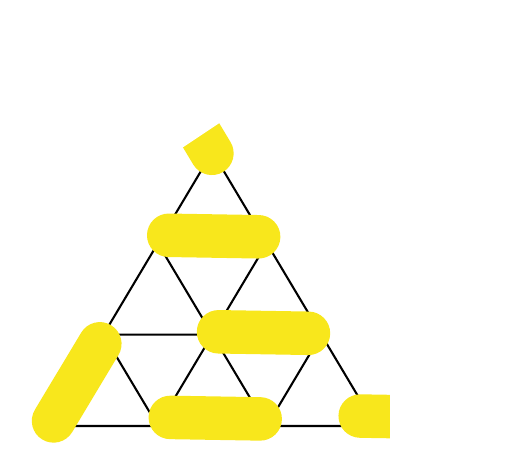
\begin{tikzpicture}[x=0.75pt,y=0.75pt,yscale=-0.75,xscale=0.75]
%uncomment if require: \path (0,300); %set diagram left start at 0, and has height of 300

%Shape: Triangle [id:dp5394198004259025] 
\draw   (272,182.33) -- (307,241) -- (237,241) -- cycle ;
%Shape: Triangle [id:dp0060243569953495335] 
\draw   (202,182.33) -- (237,241) -- (167,241) -- cycle ;
%Shape: Triangle [id:dp5009006316084215] 
\draw   (237,123.66) -- (272,182.33) -- (202,182.33) -- cycle ;
%Shape: Triangle [id:dp5954923975464252] 
\draw   (342,182.33) -- (377,241) -- (307,241) -- cycle ;
%Shape: Triangle [id:dp9717966554343387] 
\draw   (307,123.66) -- (342,182.33) -- (272,182.33) -- cycle ;
%Shape: Triangle [id:dp29175836331511373] 
\draw   (272,64.99) -- (307,123.66) -- (237,123.66) -- cycle ;
%Rounded Rect [id:dp9303927185789262] 
\draw  [draw opacity=0][fill={rgb, 255:red, 248; green, 231; blue, 28 }  ,fill opacity=1 ] (162.79,249.71) .. controls (156.17,245.74) and (154.03,237.15) .. (158,230.54) -- (187.75,181.02) .. controls (191.72,174.4) and (200.3,172.26) .. (206.92,176.24) -- (206.92,176.24) .. controls (213.53,180.21) and (215.67,188.79) .. (211.7,195.41) -- (181.96,244.92) .. controls (177.99,251.54) and (169.4,253.68) .. (162.79,249.71) -- cycle ;
%Rounded Rect [id:dp2973774835771079] 
\draw  [draw opacity=0][fill={rgb, 255:red, 248; green, 231; blue, 28 }  ,fill opacity=1 ] (230.01,118.26) .. controls (230.13,110.55) and (236.49,104.4) .. (244.21,104.52) -- (301.96,105.48) .. controls (309.68,105.61) and (315.83,111.97) .. (315.7,119.68) -- (315.7,119.68) .. controls (315.57,127.4) and (309.21,133.55) .. (301.5,133.42) -- (243.74,132.46) .. controls (236.03,132.34) and (229.88,125.98) .. (230.01,118.26) -- cycle ;
%Rounded Rect [id:dp7712557322954827] 
\draw  [draw opacity=0][fill={rgb, 255:red, 248; green, 231; blue, 28 }  ,fill opacity=1 ] (231.01,235.26) .. controls (231.13,227.55) and (237.49,221.4) .. (245.21,221.52) -- (302.96,222.48) .. controls (310.68,222.61) and (316.83,228.97) .. (316.7,236.68) -- (316.7,236.68) .. controls (316.57,244.4) and (310.21,250.55) .. (302.5,250.42) -- (244.74,249.46) .. controls (237.03,249.34) and (230.88,242.98) .. (231.01,235.26) -- cycle ;
%Rounded Rect [id:dp25009751823087134] 
\draw  [draw opacity=0][fill={rgb, 255:red, 248; green, 231; blue, 28 }  ,fill opacity=1 ] (262.01,180.26) .. controls (262.13,172.55) and (268.49,166.4) .. (276.21,166.52) -- (333.96,167.48) .. controls (341.68,167.61) and (347.83,173.97) .. (347.7,181.68) -- (347.7,181.68) .. controls (347.57,189.4) and (341.21,195.55) .. (333.5,195.42) -- (275.74,194.46) .. controls (268.03,194.34) and (261.88,187.98) .. (262.01,180.26) -- cycle ;
%Rounded Rect [id:dp12607246135910644] 
\draw  [draw opacity=0][fill={rgb, 255:red, 248; green, 231; blue, 28 }  ,fill opacity=1 ] (353.01,234.39) .. controls (353.13,226.67) and (359.49,220.52) .. (367.21,220.65) -- (424.96,221.61) .. controls (432.68,221.73) and (438.83,228.09) .. (438.7,235.81) -- (438.7,235.81) .. controls (438.57,243.52) and (432.21,249.67) .. (424.5,249.55) -- (366.74,248.59) .. controls (359.03,248.46) and (352.88,242.1) .. (353.01,234.39) -- cycle ;
%Shape: Rectangle [id:dp4625096290080499] 
\draw  [draw opacity=0][fill={rgb, 255:red, 255; green, 255; blue, 255 }  ,fill opacity=1 ] (386,214) -- (450.71,214) -- (450.71,254) -- (386,254) -- cycle ;
%Rounded Rect [id:dp22383160699593008] 
\draw  [draw opacity=0][fill={rgb, 255:red, 248; green, 231; blue, 28 }  ,fill opacity=1 ] (234.81,4.31) .. controls (241.43,0.34) and (250.01,2.49) .. (253.98,9.11) -- (283.69,58.65) .. controls (287.66,65.26) and (285.51,73.85) .. (278.89,77.81) -- (278.89,77.81) .. controls (272.27,81.78) and (263.69,79.64) .. (259.72,73.02) -- (230.02,23.48) .. controls (226.05,16.86) and (228.2,8.28) .. (234.81,4.31) -- cycle ;
%Shape: Rectangle [id:dp768095676065814] 
\draw  [draw opacity=0][fill={rgb, 255:red, 255; green, 255; blue, 255 }  ,fill opacity=1 ] (246.79,66.21) -- (207.94,7.98) -- (241.21,-14.21) -- (280.06,44.02) -- cycle ;




\end{tikzpicture}

        \label{fig:rvb-component}
    }
    \subfigure[一种低能激发态:一个自旋单态“对”被解开,产生两个向上的自旋]{
        

\tikzset{every picture/.style={line width=0.75pt}} %set default line width to 0.75pt        

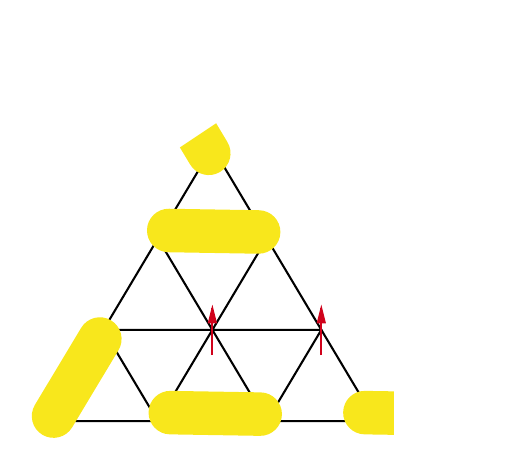
\begin{tikzpicture}[x=0.75pt,y=0.75pt,yscale=-0.75,xscale=0.75]
%uncomment if require: \path (0,300); %set diagram left start at 0, and has height of 300

%Shape: Triangle [id:dp7709012666212918] 
\draw   (292,174.46) -- (327,233.12) -- (257,233.12) -- cycle ;
%Shape: Triangle [id:dp9295040886868511] 
\draw   (222,174.46) -- (257,233.12) -- (187,233.12) -- cycle ;
%Shape: Triangle [id:dp177949788580418] 
\draw   (257,115.79) -- (292,174.46) -- (222,174.46) -- cycle ;
%Shape: Triangle [id:dp03247866415223255] 
\draw   (362,174.46) -- (397,233.12) -- (327,233.12) -- cycle ;
%Shape: Triangle [id:dp26037578632796765] 
\draw   (327,115.79) -- (362,174.46) -- (292,174.46) -- cycle ;
%Shape: Triangle [id:dp3012062348071127] 
\draw   (292,57.12) -- (327,115.79) -- (257,115.79) -- cycle ;
%Rounded Rect [id:dp4030558357818268] 
\draw  [draw opacity=0][fill={rgb, 255:red, 248; green, 231; blue, 28 }  ,fill opacity=1 ] (182.79,241.83) .. controls (176.17,237.86) and (174.03,229.28) .. (178,222.66) -- (207.75,173.14) .. controls (211.72,166.53) and (220.3,164.39) .. (226.92,168.36) -- (226.92,168.36) .. controls (233.53,172.33) and (235.67,180.92) .. (231.7,187.53) -- (201.96,237.05) .. controls (197.99,243.66) and (189.4,245.81) .. (182.79,241.83) -- cycle ;
%Rounded Rect [id:dp16737425370308645] 
\draw  [draw opacity=0][fill={rgb, 255:red, 248; green, 231; blue, 28 }  ,fill opacity=1 ] (250.01,110.39) .. controls (250.13,102.67) and (256.49,96.52) .. (264.21,96.65) -- (321.96,97.61) .. controls (329.68,97.73) and (335.83,104.09) .. (335.7,111.81) -- (335.7,111.81) .. controls (335.57,119.52) and (329.21,125.67) .. (321.5,125.55) -- (263.74,124.59) .. controls (256.03,124.46) and (249.88,118.1) .. (250.01,110.39) -- cycle ;
%Rounded Rect [id:dp7997977143532831] 
\draw  [draw opacity=0][fill={rgb, 255:red, 248; green, 231; blue, 28 }  ,fill opacity=1 ] (251.01,227.39) .. controls (251.13,219.67) and (257.49,213.52) .. (265.21,213.65) -- (322.96,214.61) .. controls (330.68,214.73) and (336.83,221.09) .. (336.7,228.81) -- (336.7,228.81) .. controls (336.57,236.52) and (330.21,242.67) .. (322.5,242.55) -- (264.74,241.59) .. controls (257.03,241.46) and (250.88,235.1) .. (251.01,227.39) -- cycle ;
%Straight Lines [id:da8204619655647556] 
\draw [color={rgb, 255:red, 208; green, 2; blue, 27 }  ,draw opacity=1 ]   (292,190.68) -- (292,160.23) ;
\draw [shift={(292,158.23)}, rotate = 450] [fill={rgb, 255:red, 208; green, 2; blue, 27 }  ,fill opacity=1 ][line width=0.08]  [draw opacity=0] (12,-3) -- (0,0) -- (12,3) -- cycle    ;
%Straight Lines [id:da301443667677862] 
\draw [color={rgb, 255:red, 208; green, 2; blue, 27 }  ,draw opacity=1 ]   (362,190.68) -- (362,160.23) ;
\draw [shift={(362,158.23)}, rotate = 450] [fill={rgb, 255:red, 208; green, 2; blue, 27 }  ,fill opacity=1 ][line width=0.08]  [draw opacity=0] (12,-3) -- (0,0) -- (12,3) -- cycle    ;
%Rounded Rect [id:dp28390331250432066] 
\draw  [draw opacity=0][fill={rgb, 255:red, 248; green, 231; blue, 28 }  ,fill opacity=1 ] (376.01,227.39) .. controls (376.13,219.67) and (382.49,213.52) .. (390.21,213.65) -- (447.96,214.61) .. controls (455.68,214.73) and (461.83,221.09) .. (461.7,228.81) -- (461.7,228.81) .. controls (461.57,236.52) and (455.21,242.67) .. (447.5,242.55) -- (389.74,241.59) .. controls (382.03,241.46) and (375.88,235.1) .. (376.01,227.39) -- cycle ;
%Shape: Rectangle [id:dp4527570591753749] 
\draw  [draw opacity=0][fill={rgb, 255:red, 255; green, 255; blue, 255 }  ,fill opacity=1 ] (409,207) -- (473.71,207) -- (473.71,247) -- (409,247) -- cycle ;
%Rounded Rect [id:dp3963770711962662] 
\draw  [draw opacity=0][fill={rgb, 255:red, 248; green, 231; blue, 28 }  ,fill opacity=1 ] (252.81,-0.47) .. controls (259.43,-4.44) and (268.01,-2.29) .. (271.98,4.32) -- (301.69,53.86) .. controls (305.66,60.48) and (303.51,69.06) .. (296.89,73.03) -- (296.89,73.03) .. controls (290.27,77) and (281.69,74.85) .. (277.72,68.23) -- (248.02,18.69) .. controls (244.05,12.08) and (246.2,3.49) .. (252.81,-0.47) -- cycle ;
%Shape: Rectangle [id:dp5531026767203489] 
\draw  [draw opacity=0][fill={rgb, 255:red, 255; green, 255; blue, 255 }  ,fill opacity=1 ] (264.79,61.43) -- (225.94,3.2) -- (259.21,-19) -- (298.06,39.23) -- cycle ;




\end{tikzpicture}

        \label{fig:rvb-up-excitation}
    }
    \caption{RVB态及其元激发}
\end{figure}

现在我们分析RVB态之上的元激发。将相邻的两个自旋当成一个自由度,则它可以分解为
\begin{equation}
    \frac{1}{2} \otimes \frac{1}{2} = 0 \oplus 1,
\end{equation}
RVB态中,像\autoref{fig:rvb-component}中这样被同一块黄色区域覆盖的两个格点占据上式中的单态,那么可以给系统一个局域的激励,让某一对最近邻格点的状态变成一个自旋三重态。
\autoref{fig:rvb-up-excitation}展示了一种这样的激发态:一个$(\ket*{\uparrow \downarrow} - \ket*{\downarrow \uparrow}) / \sqrt{2}$态被激发成$\ket*{\uparrow \uparrow}$,图形化地展示就是。
组成自旋三态的两个自旋可以跑:我们总是可以重新安排自旋配对,于是我们可以认为自旋$1$的激发被拆成了两半,每一个都可以四处移动。这就得到了\concept{自旋子(spinon)}。
可以验证这是费米子,
这些自旋子全部都是自旋$1/2$的,并且总是有偶数个自旋子。

因此,至少有一类自旋系统——基态为RVB态的自旋液体——中可以演生出费米子激发,这让我们有理由相信,做费米型的部分子拆分至少对一些自旋系统是合理的。

\subsubsection{slave boson方法}

我们对海森堡模型使用\concept{slave boson}方法,这是指做分解
\begin{equation}
    {S}_{\vb*{i}} = \frac{1}{2} {f}_{\vb*{i} \alpha}^\dagger \vb*{\sigma}_{\alpha \beta} f_{\vb*{i} \beta},
\end{equation}
其中${f}$为费米子;每个格点上的自旋的取值由这个格点上的费米型部分子的自旋携带。
这个方法本来是用于分析携带电荷的费米子的,但是后来被用在了分析自旋上,相应的这种方法分解出来的部分子在自旋系统中就是费米子而不是玻色子。
使用费米型部分子的好处在于可以避免玻色子陷入玻色-爱因斯坦凝聚态;如果自旋系统中的元激发实际上并不处在玻色-爱因斯坦凝聚态,这就意味着我们需要某种很强的玻色型部分子之间的相互作用让玻色-爱因斯坦凝聚态不稳定,即需要很强的量子涨落,于是我们无非是把一个强关联问题转化成了另一个强关联问题。
但是,如前所述,RVB态附近的激发真的好像一个费米子,所以我们有理由相信,如果在某个晶格上海森堡模型\eqref{eq:heisenberg-model-spin-liquid}真的演生出了基态是RVB态的自旋液体,那么slave boson构造就是合理的。

\subsection{费米子哈密顿量和演生$U(1)$规范场}

\subsubsection{受约束的费米子哈密顿量}

做了slave boson分解之后,哈密顿量就成为一个四阶项,描述了两个费米子的散射,写出来是
\[
    {H} = \frac{J}{4} \sum_{\pair{\vb*{i}, \vb*{j}}} (2 {f}^\dagger_{\vb*{i} \alpha} {f}_{\vb*{i} \beta} {f}_{\vb*{j} \beta}^\dagger {f}_{\vb*{j} \alpha} - {f}^\dagger_{\vb*{i} \alpha} {f}_{\vb*{i} \alpha} {f}^\dagger_{\vb*{j} \beta} {f}_{\vb*{j} \beta}),
\]
第二项由于我们要求每个格点只有单占据而可以略去,于是
\begin{equation}
    {H} = - \frac{J}{2} \sum_{\pair{\vb*{i}, \vb*{j}}} {f}_{\vb*{i} \alpha}^\dagger {f}_{\vb*{j} \beta}^\dagger {f}_{\vb*{i} \beta} {f}_{\vb*{j} \alpha}.
    \label{eq:slave-boson-hamiltonian}
\end{equation}
这个哈密顿量所在的希尔伯特空间是每个格点上有且只有一个费米子的这部分空间,写成公式就是
\begin{equation}
    f_{\vb*{i} \alpha}^\dagger f_{\vb*{j} \alpha} = 1, 
    \label{eq:one-site-one-fermion}
\end{equation}
注意其中$\vb*{i}$不求和而$\alpha$求和。
这个约束在接下来的计算中必须始终被考虑到,它的一个直接推论是
\begin{equation}
    \epsilon_{\alpha \beta} f_{\vb*{i} \alpha} f_{\vb*{i} \beta} = 0.
\end{equation}
\eqref{eq:slave-boson-hamiltonian}本身不会将一个满足\eqref{eq:one-site-one-fermion}的态转化成一个不满足这一限制的态,因此这里没有任何矛盾。

\subsubsection{路径积分和演生规范场}

下面我们使用路径积分方法引入约束\eqref{eq:one-site-one-fermion}。使用一个逐点的拉格朗日乘子$\lambda$来施加约束条件,我们有
\begin{equation}
    S[f, \bar{f}, \lambda] = \int_0^\beta \dd{\tau} \left( \sum_{\vb*{i}} \bar{f}_{\vb*{i} \alpha} \partial_\tau f_{\vb*{i} \alpha} + \sum_{\vb*{i}} \ii \lambda_{\vb*{i}} (\bar{f}_{\vb*{i} \alpha} f_{\vb*{i} \alpha} - 1) - \frac{J}{2} \sum_{\pair{\vb*{i}, \vb*{j}}} \bar{f}_{\vb*{i} \alpha} \bar{f}_{\vb*{j} \beta} f_{\vb*{j} \alpha} f_{\vb*{i} \beta} \right).
    \label{eq:spin-liquid-action}
\end{equation}
积掉拉格朗日乘子$\lambda_{\vb*{i}}$就能产生硬约束\eqref{eq:one-site-one-fermion}。

我们注意到,$\lambda_{\vb*{i}}$出现的位置和电势基本上一模一样(见\eqref{eq:imaginary-em-covariant-derivative}),且显然具有局域$U(1)$对称性。
这让我们猜测,\eqref{eq:spin-liquid-action}实际是一个自旋$1/2$费米子和某个$U(1)$规范场耦合的理论。
实际上,容易验证,将理论
\begin{equation}
    S[f, \bar{f}, \lambda, \chi, \bar{\chi}] = \int_0^\beta \dd{\tau} \left( \sum_{\vb*{i}} \bar{f}_{\vb*{i} \alpha} \partial_\tau f_{\vb*{i} \alpha} + \sum_{\vb*{i}} \ii \lambda_{\vb*{i}} (\bar{f}_{\vb*{i} \alpha} f_{\vb*{i} \alpha} - 1) + \frac{J}{2} \sum_{\pair{\vb*{i}, \vb*{j}}} (\abs{\chi_{\vb*{i} \vb*{j}}}^2 - \chi_{\vb*{i} \vb*{j}} \bar{f}_{\vb*{i} \alpha} f_{\vb*{j} \alpha} + \text{h.c.}) \right)
\end{equation}
积掉$\chi$,得到的正是\eqref{eq:spin-liquid-action}。
上式对应的哈密顿量是(注意)
\begin{equation}
    H = 
\end{equation}

如果\eqref{eq:spin-liquid-action}有非平庸的鞍点解,它附近的涨落肯定会破坏一些局域$U(1)$对称性。
现在我们假定在某些情况下可以有这样的鞍点解:$\Delta_{\vb*{i} \vb*{j}}$非零,但是$\chi_{\vb*{i} \vb*{j}}$为零。
此时
\begin{equation}
    S = \int_0^\beta \dd{\tau} \left( \sum_{\vb*{i}} \bar{f}_{\vb*{i} \alpha} (\partial_\tau - \ii \lambda_{\vb*{i}}) f_{\vb*{i} \alpha} - \tilde{J} \sum_{\pair{\vb*{i}, \vb*{j}}} \bar{\Delta}_{\vb*{i} \vb*{j}} \epsilon_{\alpha \beta} b_{\vb*{i} \alpha} b_{\vb*{j} \beta} + \text{h.c.} \right)
\end{equation}

\subsection{格点$U(1)$规范场论}

\subsubsection{平均场方法}

设
\begin{equation}
    {\Delta}_{\vb*{i} \vb*{j}} = \epsilon_{\alpha \beta} {f}_{\vb*{i} \alpha} {f}_{\vb*{j} \beta}, \quad {\chi} = {f}^\dagger_{\vb*{i} \alpha} {f}_{\vb*{j} \alpha},
\end{equation}
有
\begin{equation}
    {H} = - \frac{J}{2} \sum_{\pair{\vb*{i}, \vb*{j}}} {\Delta}^\dagger_{\vb*{i} \vb*{j}} {\Delta}_{\vb*{i} \vb*{j}} = - \frac{J}{2} \sum_{\pair{\vb*{i}, \vb*{j}}} {\chi}_{\vb*{i} \vb*{j}}^\dagger {\chi}_{\vb*{i} \vb*{j}} = - \frac{J}{4} \sum_{\pair{\vb*{i}, \vb*{j}}} ({\Delta}^\dagger_{\vb*{i} \vb*{j}} {\Delta}_{\vb*{i} \vb*{j}} + {\chi}^\dagger_{\vb*{i} \vb*{j}} {\chi}_{\vb*{i} \vb*{j}}),
\end{equation}
于是可以对最后一个形式做平均场近似;我们引入了两个参量,为了增加变分计算的参数,使之更加有效。
直接做平均场分解,有(我们将算符的期望值去掉帽子)
\[
    {H}_\text{MF} = - \frac{J}{4} \sum_{\pair{\vb*{i}, \vb*{j}}} (\Delta_{\vb*{i} \vb*{j}}^* {\Delta}_{\vb*{i} \vb*{j}} + {\Delta}_{\vb*{i} \vb*{j}} \Delta_{\vb*{i} \vb*{j}} - \abs*{\Delta_{\vb*{i} \vb*{j}}}^2) - \frac{J}{4} \sum_{\pair{\vb*{i}, \vb*{j}}} (\chi_{\vb*{i} \vb*{j}}^* {\chi}_{\vb*{i} \vb*{j}} + {\chi}_{\vb*{i} \vb*{j}} \chi_{\vb*{i} \vb*{j}} - \abs*{\chi_{\vb*{i} \vb*{j}}}^2).
\]
但是,实际上应该将系数设置成$3/8$,因为数值计算说明,直接做平均场近似效果非常糟糕。我们下面将会将系数统一称为$\tilde{J}$。
实际上严格计算平均场理论并没有什么意义,因为平均场理论的定量结果向来是非常糟糕的,而使用变分蒙特卡洛方法不难得到较为精确的结果。

原则上我们可以从平均场理论出发,通过一些方法——如大$N$展开,这里$N=2$——计算更高阶修正,但是这样非常繁琐,而仅计算有限阶可能效果也不好。

我们很关心演生规范场是不是禁闭的,如果是的话,它将不会有任何物理效应,因为低能下不会出现任何规范场涨落,而如果能量足够高,那就不再能够“只考虑基态附近的涨落”。

在格点规范场中允许存在磁单极子;此时它称为\concept{紧致的规范场},因为规范群是紧致的。
实际上,电动力学在格点上的规范群并不是$U(1)$的,因为$0$和$2\pi$不等价。

还有一种拆分方式:slave fermion,即Schwinger boson

参考: RMP 78 17 2006

\subsection{元激发和拓扑序}

举例:Resonance Valence Bond state : superposition of all pairing configurations, not a product state
看到一个

spin singlet pairs

但是,这就得到了spinon
有$\mathbb{Z}_2$-charge, so there are $\mathbb{Z}_2$-vortices.

TODO:为什么能够认为

Since $e$ and $m$ determines remaining states

spinon must carry a half-integer spin, and odd  of spoinons 

flux-fusion anomaly test

vison带有整数自旋(由于只区分拓扑性质,可以认为vison不带自旋,因为带有自旋的vison可以分解成一个带有自旋的平凡的激发和一个不带有自旋的vison激发)

Insertion of 

LSM theorem: if in each unit cell of a system there are odd spin-$1/2$, there must be ground state degeneracy.

possible phases:

\begin{enumerate}
    \item Trivial paramagnet: no ground state degeneracy
    \item Symmetry-breaking phases: FM, AFM, VBS, etc. Ground state degeneracy due to symmetry breaking.
    \item GSD on a torus, due to topological order
    \item GSD due to gapless excitations / 
\end{enumerate}

The theorem and the boundary of a topological state look quite alike, and this is not coincidence.

spin-1/2 edge of a spin AKLT chain

\subsection{演生规范场}

严格来说,此时做平均场是有问题的,因为我们手动地破缺了每个格点上粒子数始终唯一的限制,但是实际上,由于这个费米子模型实际上是一个自旋模型,这样的破缺是不正确的。
为此需要加入一个拉格朗日乘子项来固定每个格点上的粒子数,具体的拉格朗日乘子大小不能确定,是路径积分中需要额外做积分的一个场变量。

总之,在做平均场近似时我们得到了一个演生的规范场。

RMP 51, 657, 1979

总之,我们到现在用到了这些激发:我们观察到自旋液体系统中会有玻色spinon激发,这启发我们将自旋自由度拆分成玻色子,期望能够得到一个关于spinon激发的有效理论。
对拆分完成后的哈密顿量做约束以要求格点上玻色子单占据,并作平均场理论,我们得到一个规范场理论,拆分出的玻色子是物质场,还有一个定义在格子的边上的规范联络。
我们分析这个演生规范场,积掉spinon激发(实际上是自旋自由度拆分出的玻色子,我们相信它具有spinon的意义),得到一个纯粹的规范场理论(其中有动力学未给定的规范荷,可以据此定性分析spinon和规范场的相互作用),并发现这个规范场理论对应一个横场伊辛模型,它的铁磁相对应一个禁闭相,其中

\subsection{自旋液体中的对称性分数化}

大部分对称性都有所谓的对称性反常,需要生存在高维SPT(??)的边界态上。
直接从对称性分析出发可以得到大量的态,但是满足一定非常合理的条件的态是很少的,这些态均可以直接使用平均场构造出来。

Tensor category group cohomology(??)

边界和bulk上中的态都

\section{Toric-code模型}

\subsection{Toric-code哈密顿量与解析解}

Kitaev最早提出了一种模型,作为一种可能的量子计算纠错编码,他发现这个模型放在一个环面上可以有非常有趣的结果。
然而,事后发现这个模型实际上展现出了一个拓扑序。

\begin{figure}
    \centering
    \subfigure[Toric-code模型的希尔伯特空间的一组基底由这样的态构成:每条边上都或是有确定的$\sigma^z$或是有确定的$\sigma^x$]{
        \documentclass[hyperref, UTF8, a4paper]{ctexart}

\usepackage{geometry}
\usepackage{titling}
\usepackage{titlesec}
\usepackage{paralist}
\usepackage{footnote}
\usepackage{enumerate}
\usepackage{amsmath, amssymb, amsthm}
\usepackage{bbm}
\usepackage{cite}
\usepackage{graphicx}
\usepackage{subfigure}
\usepackage{physics}
\usepackage{tikz}
\usepackage{autobreak}
\usepackage[ruled, vlined, linesnumbered, noend]{algorithm2e}
\usepackage[colorlinks, linkcolor=black, anchorcolor=black, citecolor=black]{hyperref}
\usepackage{prettyref}

% Page style
\geometry{left=3.18cm,right=3.18cm,top=2.54cm,bottom=2.54cm}
\titlespacing{\paragraph}{0pt}{1pt}{10pt}[20pt]
\setlength{\droptitle}{-5em}
\preauthor{\vspace{-10pt}\begin{center}}
\postauthor{\par\end{center}}

% Math operators
\DeclareMathOperator{\timeorder}{T}
\DeclareMathOperator{\diag}{diag}
\DeclareMathOperator{\legpoly}{P}
\DeclareMathOperator{\primevalue}{P}
\DeclareMathOperator{\sgn}{sgn}
\newcommand*{\ii}{\mathrm{i}}
\newcommand*{\ee}{\mathrm{e}}
\newcommand*{\const}{\mathrm{const}}
\newcommand*{\comment}{\paragraph{注记}}
\newcommand*{\suchthat}{\quad \text{s.t.} \quad}
\newcommand*{\argmin}{\arg\min}
\newcommand*{\argmax}{\arg\max}
\newcommand*{\normalorder}[1]{: #1 :}
\newcommand*{\pair}[1]{\langle #1 \rangle}
\newcommand*{\fd}[1]{\mathcal{D} #1}
\DeclareMathOperator{\bigO}{\mathcal{O}}

% prettyref setting
\newrefformat{sec}{第\ref{#1}节}
\newrefformat{note}{注\ref{#1}}
\newrefformat{fig}{图\ref{#1}}
\newrefformat{alg}{算法\ref{#1}}
\renewcommand{\autoref}{\prettyref}

% TikZ setting
\usetikzlibrary{arrows,shapes,positioning}
\usetikzlibrary{arrows.meta}
\usetikzlibrary{decorations.markings}
\tikzstyle arrowstyle=[scale=1]
\tikzstyle directed=[postaction={decorate,decoration={markings,
    mark=at position .5 with {\arrow[arrowstyle]{stealth}}}}]
\tikzstyle ray=[directed, thick]
\tikzstyle dot=[anchor=base,fill,circle,inner sep=1pt]

% Algorithm setting
\renewcommand{\algorithmcfname}{算法}
% Python-style code
\SetKwIF{If}{ElseIf}{Else}{if}{:}{elif:}{else:}{}
\SetKwFor{For}{for}{:}{}
\SetKwFor{While}{while}{:}{}
\SetKwInput{KwData}{输入}
\SetKwInput{KwResult}{输出}
\SetArgSty{textnormal}

\renewcommand{\emph}[1]{\textbf{#1}}
\newcommand*{\concept}[1]{\underline{\textbf{#1}}}
\newcommand*{\Ztwo}{$\mathbb{Z}_2$}

\title{常见格点模型}
\author{吴何友}

\begin{document}

\maketitle

\section{相互作用体系}

\subsection{Hubbard模型}

\concept{Hubbard模型}是一种常见的强关联电子模型,它是一个定义在点阵上的模型,以下我们照惯例用$i, j$等表示格点坐标。
不包含化学势的哈密顿量为
\begin{equation}
    \hat{H} = \underbrace{-t \sum_{\pair{i, j}, \sigma} \hat{c}_{i\sigma}^\dagger \hat{c}_{j\sigma} + \text{h.c.}}_{\hat{H}_0} + \underbrace{U \sum_i \hat{n}_{i \uparrow} \hat{n}_{i \downarrow}}_{\hat{H}_\text{I}}.
\end{equation}
或者,为了后面蒙特卡洛模拟的方便,重新定义化学势,也可以有
\begin{equation}
    \hat{H} = -t \sum_{\pair{i, j}, \sigma} \hat{c}_{i\sigma}^\dagger \hat{c}_{j\sigma} + \text{h.c.} 
    + U \sum_i \left(\hat{n}_{i\uparrow} - \frac{1}{2}\right) \left(\hat{n}_{i\downarrow} - \frac{1}{2}\right).
\end{equation}

\subsubsection{Hubbard模型的量子蒙特卡洛模拟}

\subsection{Trotter分解和辅助场引入}

下面我们尝试对Hubbard模型做Trotter分解。设虚时间间隔为$\Delta\tau$,总共有$m$个虚时间点,$\tau=m\Delta \tau$。
对Hubbard模型,有一种特殊的分解方法:
\begin{equation}
    \ee^{-\Delta \tau \hat{H}_\text{I}} = \gamma \sum_{s_1, s_2, \ldots, s_N = \pm 1} \ee^{\alpha \sum_i s_i (\hat{n}_{i\uparrow} - \hat{n}_{i \downarrow})}, 
    \quad \gamma = \frac{1}{2^N} \ee^{\Delta \tau U N / 4}, \quad \cosh(\alpha) = \ee^{\Delta \tau U / 2},
\end{equation}
可以看到$\gamma$是一个和辅助场$\{s_i\}$(照惯例我们下面记它的时间线为$\vb{s}$)无关的量,考虑到配分函数的常数因子无关紧要,略去此因子,则配分函数为
\[
    \begin{aligned}
        Z &= \trace \prod_{n=1}^m \sum_{\vb{s}_{n}} \ee^{\alpha \sum_i s_i (\hat{n}_{i\uparrow} - \hat{n}_{i \downarrow})} \ee^{\Delta \tau t \sum_{\pair{i, j}, \sigma} \hat{c}_{i\sigma}^\dagger \hat{c}_{j\sigma} + \text{h.c.}} \\
        &= \sum_{\vb{s}} \prod_{n=1}^m \ee^{\alpha \hat{c}^\dagger_{\uparrow} \diag{\vb{s}_n} \hat{c}_{\uparrow}} \ee^{- \alpha \hat{c}^\dagger_{\downarrow} \diag{\vb{s}_n} \hat{c}_{\downarrow}} \ee^{- \Delta \tau \hat{c}_\uparrow^\dagger \vb{T} \hat{c}_\uparrow} \ee^{- \Delta \tau \hat{c}_\downarrow^\dagger \vb{T} \hat{c}_\downarrow},
    \end{aligned}
\]
其中我们指定$\vb{T}$是动能部分$\hat{H}_0$在单粒子表象下的系数矩阵,即
\begin{equation}
    T_{ij} = \begin{cases}
        -t, \quad &\pair{i, j}, \\
        0, \quad &\text{otherwise}.
    \end{cases}
\end{equation}
应用公式
\begin{equation}
    \trace(\ee^{- \sum_{i, j} \hat{c}_i^\dagger A_{ij} \hat{c}_j} \ee^{- \sum_{i, j} \hat{c}_i^\dagger B_{ij} \hat{c}_j} \cdots) = \det(1 + \ee^{- \vb{A}}\ee^{- \vb{B}} \cdots),
    \label{eq:trace-to-det}
\end{equation}
我们积掉费米子自由度,得到
\[
    Z = \sum_{\vb{s}} \det(1 + \prod_{n=1}^m \exp(\alpha \diag{\vb{s}_n \oplus (-\vb{s}_n)}) \exp( -\Delta \tau \pmqty{\dmat{\vb{T}, \vb{T}}})).
\]
上式中出现了矩阵拼接,因为电子的量子数同时包括位置和自旋,因此需要$2N \times 2N$的矩阵(在$2N$维中,前$N$维对应自旋向上的态,后$N$维对应自旋向下的态)。
然而,Hubbard模型的自选旋转不变性意味着以上矩阵是分块对角的,从而可以拆分开来,得到下式:
\begin{equation}
    Z = \det(1 + \prod_{\sigma=\uparrow, \downarrow} \prod_{n=1}^m \vb{B}_{\vb{s}}^\sigma(\tau) ),
\end{equation}
其中
\begin{equation}
    \vb{B}^\uparrow_{\vb{s}}(\tau) = \ee^{\alpha \diag \vb{s}_n} \ee^{-\Delta \tau \vb{T}}, \quad \vb{B}^\downarrow_{\vb{s}}(\tau) = \ee^{- \alpha \diag \vb{s}_n} \ee^{-\Delta \tau \vb{T}}.
\end{equation}
所有$\vb{B}_{\sigma}$都是一个$N \times N$矩阵,而不是$2N \times 2N$的矩阵。

\section{磁场}

将电子和一个满足库伦规范的磁矢势$\vb*{A}$耦合,那么会出现动量的一个修正,这个修在在波函数上引入如下的相位变化:
\begin{equation}
    \theta = \int \dd{\vb*{l}} \cdot \vb*{A}.
\end{equation}
在格点模型中,电子仅仅出现在格点上。我们知道紧束缚模型的哈密顿量(即跃迁项)实际上就是动能,因此加入磁场意味着紧束缚模型的$t_{ij}$出现变化,考虑相位变化,则磁场会导致以下修正:
\begin{equation}
    t_{ij} \longrightarrow \ee^{\ii e \int_j^i \dd{\vb*{l}} \cdot \vb*{A} } t_{ij}.
\end{equation}
相应的,设一个格点上的闭合路径为$C$,通过它的磁通量为$\Phi$,则
\begin{equation}
    \ee^{\ii \Phi} = \prod_{C} t_{ij}.
\end{equation}

\end{document}
    }
    \subfigure[$A$激发定义在格点上,上图是一个$A$激发的例子]{
        

\tikzset{every picture/.style={line width=0.75pt}} %set default line width to 0.75pt        

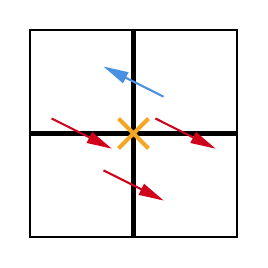
\begin{tikzpicture}[x=0.75pt,y=0.75pt,yscale=-1,xscale=1]
%uncomment if require: \path (0,300); %set diagram left start at 0, and has height of 300

%Shape: Square [id:dp6654025093743159] 
\draw   (140,67) -- (190,67) -- (190,117) -- (140,117) -- cycle ;
%Shape: Square [id:dp6286524465515233] 
\draw   (190,67) -- (240,67) -- (240,117) -- (190,117) -- cycle ;
%Shape: Square [id:dp6519468109347835] 
\draw   (140,117) -- (190,117) -- (190,167) -- (140,167) -- cycle ;
%Shape: Square [id:dp2265935355822739] 
\draw   (190,117) -- (240,117) -- (240,167) -- (190,167) -- cycle ;
%Straight Lines [id:da21658691245720751] 
\draw [line width=1.5]    (190,67) -- (190,117) ;
%Straight Lines [id:da3177017321913107] 
\draw [line width=1.5]    (140,117) -- (190,117) ;
%Straight Lines [id:da01915738195349781] 
\draw [line width=1.5]    (190,117) -- (190,167) ;
%Straight Lines [id:da717616113838583] 
\draw [line width=1.5]    (190,117) -- (240,117) ;
%Straight Lines [id:da8258680195288246] 
\draw [color={rgb, 255:red, 245; green, 166; blue, 35 }  ,draw opacity=1 ][line width=1.5]    (190,117) ;
\draw [shift={(190,117)}, rotate = 45] [color={rgb, 255:red, 245; green, 166; blue, 35 }  ,draw opacity=1 ][line width=1.5]    (-10.17,0) -- (10.17,0)(0,10.17) -- (0,-10.17)   ;
%Straight Lines [id:da10440190731652677] 
\draw [color={rgb, 255:red, 208; green, 2; blue, 27 }  ,draw opacity=1 ]   (200.54,109.75) -- (227.67,123.35) ;
\draw [shift={(229.46,124.25)}, rotate = 206.63] [fill={rgb, 255:red, 208; green, 2; blue, 27 }  ,fill opacity=1 ][line width=0.08]  [draw opacity=0] (12,-3) -- (0,0) -- (12,3) -- cycle    ;
%Straight Lines [id:da6468653685487751] 
\draw [color={rgb, 255:red, 74; green, 144; blue, 226 }  ,draw opacity=1 ]   (204.46,99.25) -- (177.33,85.65) ;
\draw [shift={(175.54,84.75)}, rotate = 386.63] [fill={rgb, 255:red, 74; green, 144; blue, 226 }  ,fill opacity=1 ][line width=0.08]  [draw opacity=0] (12,-3) -- (0,0) -- (12,3) -- cycle    ;
%Straight Lines [id:da7493786508982636] 
\draw [color={rgb, 255:red, 208; green, 2; blue, 27 }  ,draw opacity=1 ]   (175.54,134.75) -- (202.67,148.35) ;
\draw [shift={(204.46,149.25)}, rotate = 206.63] [fill={rgb, 255:red, 208; green, 2; blue, 27 }  ,fill opacity=1 ][line width=0.08]  [draw opacity=0] (12,-3) -- (0,0) -- (12,3) -- cycle    ;
%Straight Lines [id:da32966501733867193] 
\draw [color={rgb, 255:red, 208; green, 2; blue, 27 }  ,draw opacity=1 ]   (150.54,109.75) -- (177.67,123.35) ;
\draw [shift={(179.46,124.25)}, rotate = 206.63] [fill={rgb, 255:red, 208; green, 2; blue, 27 }  ,fill opacity=1 ][line width=0.08]  [draw opacity=0] (12,-3) -- (0,0) -- (12,3) -- cycle    ;




\end{tikzpicture}
      
    }
    \vfill
    \subfigure[$B$激发定义在正方形方块上,上图是一个$B$激发的例子]{
        

\tikzset{every picture/.style={line width=0.75pt}} %set default line width to 0.75pt        

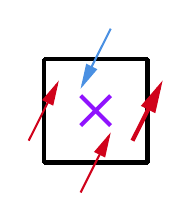
\begin{tikzpicture}[x=0.75pt,y=0.75pt,yscale=-1,xscale=1]
%uncomment if require: \path (0,300); %set diagram left start at 0, and has height of 300

%Shape: Square [id:dp06008287812795965] 
\draw   (192,54) -- (242,54) -- (242,104) -- (192,104) -- cycle ;
%Straight Lines [id:da5345790011660227] 
\draw [line width=1.5]    (192,54) -- (192,104) ;
%Straight Lines [id:da8934908293124699] 
\draw [line width=1.5]    (242,54) -- (242,104) ;
%Straight Lines [id:da6163816696768483] 
\draw [line width=1.5]    (192,54) -- (242,54) ;
%Straight Lines [id:da13968764975578463] 
\draw [line width=1.5]    (192,104) -- (242,104) ;
%Straight Lines [id:da6360739318940407] 
\draw [color={rgb, 255:red, 208; green, 2; blue, 27 }  ,draw opacity=1 ]   (184.75,93.46) -- (198.35,66.33) ;
\draw [shift={(199.25,64.54)}, rotate = 476.63] [fill={rgb, 255:red, 208; green, 2; blue, 27 }  ,fill opacity=1 ][line width=0.08]  [draw opacity=0] (12,-3) -- (0,0) -- (12,3) -- cycle    ;
%Straight Lines [id:da2436020984695373] 
\draw [color={rgb, 255:red, 74; green, 144; blue, 226 }  ,draw opacity=1 ]   (224.25,39.54) -- (210.65,66.67) ;
\draw [shift={(209.75,68.46)}, rotate = 296.63] [fill={rgb, 255:red, 74; green, 144; blue, 226 }  ,fill opacity=1 ][line width=0.08]  [draw opacity=0] (12,-3) -- (0,0) -- (12,3) -- cycle    ;
%Straight Lines [id:da6361964039179109] 
\draw [color={rgb, 255:red, 208; green, 2; blue, 27 }  ,draw opacity=1 ][line width=1.5]    (234.75,93.46) -- (247.46,68.12) ;
\draw [shift={(249.25,64.54)}, rotate = 476.63] [fill={rgb, 255:red, 208; green, 2; blue, 27 }  ,fill opacity=1 ][line width=0.08]  [draw opacity=0] (15.6,-3.9) -- (0,0) -- (15.6,3.9) -- cycle    ;
%Straight Lines [id:da7397146382660318] 
\draw [color={rgb, 255:red, 208; green, 2; blue, 27 }  ,draw opacity=1 ]   (209.75,118.46) -- (223.35,91.33) ;
\draw [shift={(224.25,89.54)}, rotate = 476.63] [fill={rgb, 255:red, 208; green, 2; blue, 27 }  ,fill opacity=1 ][line width=0.08]  [draw opacity=0] (12,-3) -- (0,0) -- (12,3) -- cycle    ;
%Straight Lines [id:da059453193677352134] 
\draw [color={rgb, 255:red, 144; green, 19; blue, 254 }  ,draw opacity=1 ][line width=1.5]    (217,79) ;
\draw [shift={(217,79)}, rotate = 45] [color={rgb, 255:red, 144; green, 19; blue, 254 }  ,draw opacity=1 ][line width=1.5]    (-10.17,0) -- (10.17,0)(0,10.17) -- (0,-10.17)   ;




\end{tikzpicture}
    }
    \subfigure[虽然$\sigma^x$和$\sigma^z$之间有量子涨落,但是$A$和$B$对易,从而系统的能量本征态可以用$A$激发和$B$激发标记;通过数自由度会发现也只需要这两个标记]{
        

\tikzset{every picture/.style={line width=0.75pt}} %set default line width to 0.75pt        

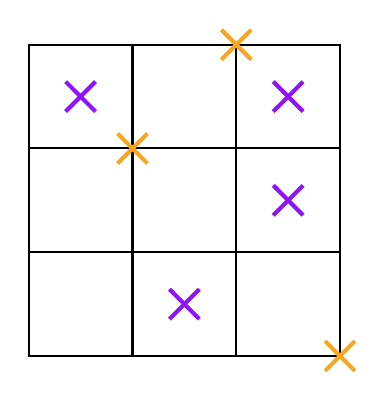
\begin{tikzpicture}[x=0.75pt,y=0.75pt,yscale=-1,xscale=1]
%uncomment if require: \path (0,300); %set diagram left start at 0, and has height of 300

%Shape: Square [id:dp4570817602982631] 
\draw   (100,29) -- (150,29) -- (150,79) -- (100,79) -- cycle ;
%Shape: Square [id:dp2903299358971252] 
\draw   (150,29) -- (200,29) -- (200,79) -- (150,79) -- cycle ;
%Shape: Square [id:dp8410481858286352] 
\draw   (100,79) -- (150,79) -- (150,129) -- (100,129) -- cycle ;
%Shape: Square [id:dp1117017430126368] 
\draw   (150,79) -- (200,79) -- (200,129) -- (150,129) -- cycle ;
%Shape: Square [id:dp9054195019818092] 
\draw   (200,29) -- (250,29) -- (250,79) -- (200,79) -- cycle ;
%Shape: Square [id:dp9918567360750739] 
\draw   (200,79) -- (250,79) -- (250,129) -- (200,129) -- cycle ;
%Shape: Square [id:dp6694249449139529] 
\draw   (100,129) -- (150,129) -- (150,179) -- (100,179) -- cycle ;
%Shape: Square [id:dp6467857772283392] 
\draw   (150,129) -- (200,129) -- (200,179) -- (150,179) -- cycle ;
%Shape: Square [id:dp32240121043282777] 
\draw   (200,129) -- (250,129) -- (250,179) -- (200,179) -- cycle ;
%Straight Lines [id:da5972676544083908] 
\draw [color={rgb, 255:red, 245; green, 166; blue, 35 }  ,draw opacity=1 ][line width=1.5]    (150,79) ;
\draw [shift={(150,79)}, rotate = 45] [color={rgb, 255:red, 245; green, 166; blue, 35 }  ,draw opacity=1 ][line width=1.5]    (-10.17,0) -- (10.17,0)(0,10.17) -- (0,-10.17)   ;
%Straight Lines [id:da06771970628563428] 
\draw [color={rgb, 255:red, 245; green, 166; blue, 35 }  ,draw opacity=1 ][line width=1.5]    (250,179) ;
\draw [shift={(250,179)}, rotate = 45] [color={rgb, 255:red, 245; green, 166; blue, 35 }  ,draw opacity=1 ][line width=1.5]    (-10.17,0) -- (10.17,0)(0,10.17) -- (0,-10.17)   ;
%Straight Lines [id:da1804222983474455] 
\draw [color={rgb, 255:red, 245; green, 166; blue, 35 }  ,draw opacity=1 ][line width=1.5]    (200,29) ;
\draw [shift={(200,29)}, rotate = 45] [color={rgb, 255:red, 245; green, 166; blue, 35 }  ,draw opacity=1 ][line width=1.5]    (-10.17,0) -- (10.17,0)(0,10.17) -- (0,-10.17)   ;
%Straight Lines [id:da7901030413597554] 
\draw [color={rgb, 255:red, 144; green, 19; blue, 254 }  ,draw opacity=1 ][line width=1.5]    (175,154) ;
\draw [shift={(175,154)}, rotate = 45] [color={rgb, 255:red, 144; green, 19; blue, 254 }  ,draw opacity=1 ][line width=1.5]    (-10.17,0) -- (10.17,0)(0,10.17) -- (0,-10.17)   ;
%Straight Lines [id:da37933960521297805] 
\draw [color={rgb, 255:red, 144; green, 19; blue, 254 }  ,draw opacity=1 ][line width=1.5]    (225,104) ;
\draw [shift={(225,104)}, rotate = 45] [color={rgb, 255:red, 144; green, 19; blue, 254 }  ,draw opacity=1 ][line width=1.5]    (-10.17,0) -- (10.17,0)(0,10.17) -- (0,-10.17)   ;
%Straight Lines [id:da13742234427535593] 
\draw [color={rgb, 255:red, 144; green, 19; blue, 254 }  ,draw opacity=1 ][line width=1.5]    (125,54) ;
\draw [shift={(125,54)}, rotate = 45] [color={rgb, 255:red, 144; green, 19; blue, 254 }  ,draw opacity=1 ][line width=1.5]    (-10.17,0) -- (10.17,0)(0,10.17) -- (0,-10.17)   ;
%Straight Lines [id:da5163777331330268] 
\draw [color={rgb, 255:red, 144; green, 19; blue, 254 }  ,draw opacity=1 ][line width=1.5]    (225,54) ;
\draw [shift={(225,54)}, rotate = 45] [color={rgb, 255:red, 144; green, 19; blue, 254 }  ,draw opacity=1 ][line width=1.5]    (-10.17,0) -- (10.17,0)(0,10.17) -- (0,-10.17)   ;




\end{tikzpicture}

    }
    \caption{Toric-code模型的系统构型和元激发}
\end{figure}

考虑一个正方晶格,在每条边(\emph{不是}每个格点!)上放有一个自旋$1/2$自由度。
哈密顿量为
\begin{equation}
    {H} = - \sum_s {A}_s - \sum_p {B}_p,
    \label{eq:toric-code-hamiltonian}
\end{equation}
其中下标$s$表示格点,${A}_s$指的是格点$s$周围的四条边上的$x$方向上的自旋算符的乘积,即
\begin{equation}
    {A}_s = \prod_{\vb*{i} \text{ near } s} {\sigma}_{\vb*{i}}^x,
\end{equation}
而$p$表示格点中的一个最小正方形方块,${B}_p$指的是正方形$p$的四条边上的$z$方向上的自旋算符的乘积,即
\begin{equation}
    {B}_p = \prod_\text{$\vb*{i}$ of $p$} {\sigma}_{\vb*{i}}^z.
\end{equation}

\eqref{eq:toric-code-hamiltonian}中显然有不小的量子涨落,因为有大量彼此不对易的算符。然而,我们将展示,它其实是严格可解的。
因此,Toric-code模型是一个很好的玩具模型,能够向我们展示量子涨落强烈的自旋系统的行为。

首先可以验证$\{{A}_s\}$和$\{{B}_p\}$构成一组对易稳定子(即平方为1的一组彼此对易的厄米算符),这样就有
\begin{equation}
    \comm*{{A}_s}{{H}} = \comm*{{B}_p}{{H}} = 0.
\end{equation}
另一方面,平方为1的厄米算符的本征值是$\pm 1$,于是我们就可以用它们的本征值$A_s = \pm 1$和$B_p = \pm 1$标记体系的能量本征态。
实际上,在热力学极限下只需要$\{A_s\}$和$\{B_p\}$就可以唯一地标记体系的能量本征态。
这是因为设体系有$N$个格点,那么有$4N/2=2N$条边,于是体系的希尔伯特空间的维数为$2^{2N}$。%
$s$和$p$均有$N$个,于是所有可能的$\{A_s\}$和$\{B_p\}$的组合总数为$2^N \cdot 2^N=2^{2N}$。
这样如果不考虑边界引入的微妙之处,只需要$\{A_s\}$和$\{B_p\}$就可以唯一地标记体系的能量本征态。
很容易看出体系的基态为所有$A_s$和$B_p$均为$1$的状态,于是我们可以把$A_s$和$B_p$为$-1$的情况看成激发态。这样我们就得到了\eqref{eq:toric-code-hamiltonian}的全部能量本征态,从而完全求解出了它。

显然Toric-code模型确实是自旋液体,因为其基态不具有任何经典意义上的序:我们得到的是一大堆$\sigma^x$确定的态和一大堆$\sigma^z$确定的态的线性叠加。

\subsection{环面上的情况}

为了解析求解,我们施加一个周期性边界条件,这相当于把体系放在了一个二维环面上。
此时诸$\{A_s\}$和$\{B_p\}$实际上不是彼此独立的,因为此时显然有
\[
    \prod_s {A}_s = 1,
\]
因为所有的$\{A_s\}$乘起来,每一条边被乘了两边,所以一定会得到$1$。类似的有
\[
    \prod_p {B}_p = 1.
\]
这两个方程要求
\begin{equation}
    \prod_{s} A_s = \prod_{p} B_p = 1.
    \label{eq:toric-code-pair-condition}
\end{equation}
这就意味着$A_s$激发和$B_p$激发必须成对出现,否则乘积将会是$-1$。我们将$A_s$激发称为e粒子,而将$B_p$激发称为m粒子,因为在某种意义上可以将$A_s$激发类比为电荷而将$B_p$激发理解为磁通量子。
这两种粒子的性质和空间的拓扑结构显然关系很大,因此称它们为拓扑激发。

\begin{figure}
    \centering
    \subfigure[将一个$O_\text{e}$开弦算符作用在一个元激发也没有的态上而得到的结果;弦两端出现了两个e激发]{
        

\tikzset{every picture/.style={line width=0.75pt}} %set default line width to 0.75pt        

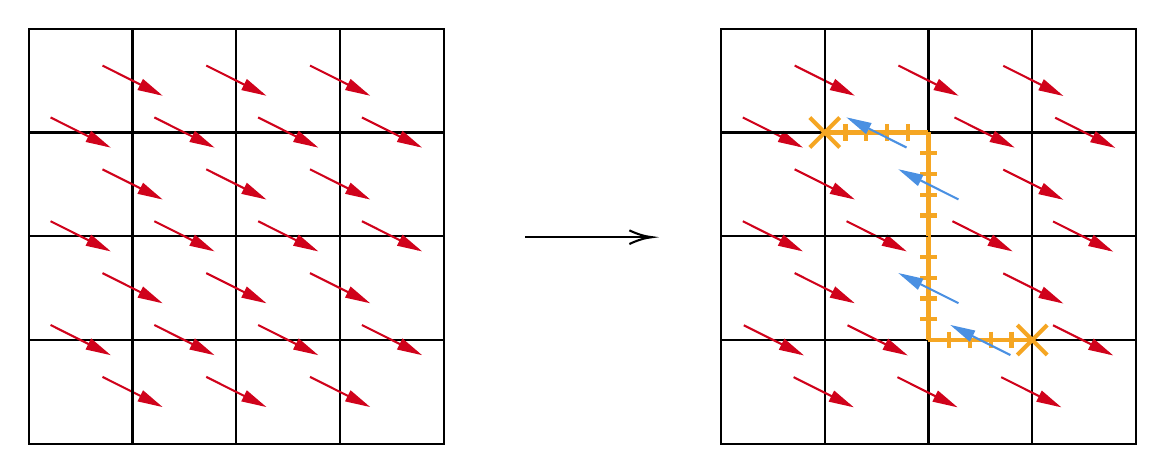
\begin{tikzpicture}[x=0.75pt,y=0.75pt,yscale=-1,xscale=1]
%uncomment if require: \path (0,300); %set diagram left start at 0, and has height of 300

%Shape: Square [id:dp3176853045406567] 
\draw   (413,192.06) -- (463,192.06) -- (463,242.06) -- (413,242.06) -- cycle ;
%Shape: Square [id:dp7022572838953951] 
\draw   (513,192.06) -- (563,192.06) -- (563,242.06) -- (513,242.06) -- cycle ;
%Shape: Square [id:dp030329102095208782] 
\draw   (513,142.06) -- (563,142.06) -- (563,192.06) -- (513,192.06) -- cycle ;
%Shape: Square [id:dp517134688980474] 
\draw   (463,192.06) -- (513,192.06) -- (513,242.06) -- (463,242.06) -- cycle ;
%Shape: Square [id:dp47682705008824966] 
\draw   (363,42.06) -- (413,42.06) -- (413,92.06) -- (363,92.06) -- cycle ;
%Shape: Square [id:dp40774233163885887] 
\draw   (413,42.06) -- (463,42.06) -- (463,92.06) -- (413,92.06) -- cycle ;
%Shape: Square [id:dp8421641317700328] 
\draw   (363,92.06) -- (413,92.06) -- (413,142.06) -- (363,142.06) -- cycle ;
%Shape: Square [id:dp8149136823625276] 
\draw   (413,92.06) -- (463,92.06) -- (463,142.06) -- (413,142.06) -- cycle ;
%Shape: Square [id:dp9420804931616191] 
\draw   (463,42.06) -- (513,42.06) -- (513,92.06) -- (463,92.06) -- cycle ;
%Shape: Square [id:dp575792276688039] 
\draw   (463,92.06) -- (513,92.06) -- (513,142.06) -- (463,142.06) -- cycle ;
%Shape: Square [id:dp604089614437928] 
\draw   (363,142.06) -- (413,142.06) -- (413,192.06) -- (363,192.06) -- cycle ;
%Shape: Square [id:dp9110252712752467] 
\draw   (413,142.06) -- (463,142.06) -- (463,192.06) -- (413,192.06) -- cycle ;
%Shape: Square [id:dp757512175683634] 
\draw   (463,142.06) -- (513,142.06) -- (513,192.06) -- (463,192.06) -- cycle ;
%Straight Lines [id:da24590588647520528] 
\draw [color={rgb, 255:red, 245; green, 166; blue, 35 }  ,draw opacity=1 ][line width=1.5]    (513,192.06) ;
\draw [shift={(513,192.06)}, rotate = 45] [color={rgb, 255:red, 245; green, 166; blue, 35 }  ,draw opacity=1 ][line width=1.5]    (-10.17,0) -- (10.17,0)(0,10.17) -- (0,-10.17)   ;
%Straight Lines [id:da734113367713265] 
\draw [color={rgb, 255:red, 245; green, 166; blue, 35 }  ,draw opacity=1 ][line width=1.5]    (463,192.06) -- (513,192.06) (473,188.06) -- (473,196.06)(483,188.06) -- (483,196.06)(493,188.06) -- (493,196.06)(503,188.06) -- (503,196.06) ;
%Straight Lines [id:da8677740521877175] 
\draw [color={rgb, 255:red, 245; green, 166; blue, 35 }  ,draw opacity=1 ][line width=1.5]    (463,192.06) -- (463,142.06) (459,182.06) -- (467,182.06)(459,172.06) -- (467,172.06)(459,162.06) -- (467,162.06)(459,152.06) -- (467,152.06) ;
%Straight Lines [id:da9217711157137525] 
\draw [color={rgb, 255:red, 208; green, 2; blue, 27 }  ,draw opacity=1 ]   (398.54,59.81) -- (425.67,73.42) ;
\draw [shift={(427.46,74.31)}, rotate = 206.63] [fill={rgb, 255:red, 208; green, 2; blue, 27 }  ,fill opacity=1 ][line width=0.08]  [draw opacity=0] (12,-3) -- (0,0) -- (12,3) -- cycle    ;
%Straight Lines [id:da8231785182807179] 
\draw    (413,42.06) -- (413,92.06) ;
%Straight Lines [id:da41308525995744727] 
\draw    (413,92.06) -- (413,142.06) ;
%Straight Lines [id:da3012120677599419] 
\draw [color={rgb, 255:red, 208; green, 2; blue, 27 }  ,draw opacity=1 ]   (373.54,84.81) -- (400.67,98.42) ;
\draw [shift={(402.46,99.31)}, rotate = 206.63] [fill={rgb, 255:red, 208; green, 2; blue, 27 }  ,fill opacity=1 ][line width=0.08]  [draw opacity=0] (12,-3) -- (0,0) -- (12,3) -- cycle    ;
%Straight Lines [id:da05997957846750057] 
\draw    (363,92.06) -- (413,92.06) ;
%Straight Lines [id:da3962017480147524] 
\draw [color={rgb, 255:red, 208; green, 2; blue, 27 }  ,draw opacity=1 ]   (398.54,109.81) -- (425.67,123.42) ;
\draw [shift={(427.46,124.31)}, rotate = 206.63] [fill={rgb, 255:red, 208; green, 2; blue, 27 }  ,fill opacity=1 ][line width=0.08]  [draw opacity=0] (12,-3) -- (0,0) -- (12,3) -- cycle    ;
%Straight Lines [id:da8887410805092772] 
\draw [color={rgb, 255:red, 74; green, 144; blue, 226 }  ,draw opacity=1 ]   (477.46,174.31) -- (450.33,160.71) ;
\draw [shift={(448.54,159.81)}, rotate = 386.63] [fill={rgb, 255:red, 74; green, 144; blue, 226 }  ,fill opacity=1 ][line width=0.08]  [draw opacity=0] (12,-3) -- (0,0) -- (12,3) -- cycle    ;
%Straight Lines [id:da3161585135502756] 
\draw [color={rgb, 255:red, 74; green, 144; blue, 226 }  ,draw opacity=1 ]   (502.46,199.31) -- (475.33,185.71) ;
\draw [shift={(473.54,184.81)}, rotate = 386.63] [fill={rgb, 255:red, 74; green, 144; blue, 226 }  ,fill opacity=1 ][line width=0.08]  [draw opacity=0] (12,-3) -- (0,0) -- (12,3) -- cycle    ;
%Straight Lines [id:da02918311398315465] 
\draw    (463,42.06) -- (463,92.06) ;
%Straight Lines [id:da2940193548924497] 
\draw [color={rgb, 255:red, 208; green, 2; blue, 27 }  ,draw opacity=1 ]   (448.54,59.81) -- (475.67,73.42) ;
\draw [shift={(477.46,74.31)}, rotate = 206.63] [fill={rgb, 255:red, 208; green, 2; blue, 27 }  ,fill opacity=1 ][line width=0.08]  [draw opacity=0] (12,-3) -- (0,0) -- (12,3) -- cycle    ;
%Straight Lines [id:da2999016051074743] 
\draw [color={rgb, 255:red, 208; green, 2; blue, 27 }  ,draw opacity=1 ]   (423.54,134.81) -- (450.67,148.42) ;
\draw [shift={(452.46,149.31)}, rotate = 206.63] [fill={rgb, 255:red, 208; green, 2; blue, 27 }  ,fill opacity=1 ][line width=0.08]  [draw opacity=0] (12,-3) -- (0,0) -- (12,3) -- cycle    ;
%Straight Lines [id:da13812102603223497] 
\draw    (413,142.06) -- (463,142.06) ;
%Straight Lines [id:da473115693085842] 
\draw [color={rgb, 255:red, 245; green, 166; blue, 35 }  ,draw opacity=1 ][line width=1.5]    (413,92.06) -- (463,92.06) (423,88.06) -- (423,96.06)(433,88.06) -- (433,96.06)(443,88.06) -- (443,96.06)(453,88.06) -- (453,96.06) ;
%Straight Lines [id:da21779160831084354] 
\draw [color={rgb, 255:red, 245; green, 166; blue, 35 }  ,draw opacity=1 ][line width=1.5]    (463,142.06) -- (463,92.06) (459,132.06) -- (467,132.06)(459,122.06) -- (467,122.06)(459,112.06) -- (467,112.06)(459,102.06) -- (467,102.06) ;
%Straight Lines [id:da08642153104428818] 
\draw    (363,142.06) -- (413,142.06) ;
%Straight Lines [id:da6951119379014274] 
\draw [color={rgb, 255:red, 208; green, 2; blue, 27 }  ,draw opacity=1 ]   (373.54,134.81) -- (400.67,148.42) ;
\draw [shift={(402.46,149.31)}, rotate = 206.63] [fill={rgb, 255:red, 208; green, 2; blue, 27 }  ,fill opacity=1 ][line width=0.08]  [draw opacity=0] (12,-3) -- (0,0) -- (12,3) -- cycle    ;
%Straight Lines [id:da08264979104155512] 
\draw    (413,142.06) -- (413,192.06) ;
%Straight Lines [id:da8129978724657629] 
\draw [color={rgb, 255:red, 208; green, 2; blue, 27 }  ,draw opacity=1 ]   (398.54,159.81) -- (425.67,173.42) ;
\draw [shift={(427.46,174.31)}, rotate = 206.63] [fill={rgb, 255:red, 208; green, 2; blue, 27 }  ,fill opacity=1 ][line width=0.08]  [draw opacity=0] (12,-3) -- (0,0) -- (12,3) -- cycle    ;
%Straight Lines [id:da16655027105891573] 
\draw [color={rgb, 255:red, 208; green, 2; blue, 27 }  ,draw opacity=1 ]   (474.54,134.81) -- (501.67,148.42) ;
\draw [shift={(503.46,149.31)}, rotate = 206.63] [fill={rgb, 255:red, 208; green, 2; blue, 27 }  ,fill opacity=1 ][line width=0.08]  [draw opacity=0] (12,-3) -- (0,0) -- (12,3) -- cycle    ;
%Straight Lines [id:da961269861360253] 
\draw [color={rgb, 255:red, 208; green, 2; blue, 27 }  ,draw opacity=1 ]   (475.54,84.81) -- (502.67,98.42) ;
\draw [shift={(504.46,99.31)}, rotate = 206.63] [fill={rgb, 255:red, 208; green, 2; blue, 27 }  ,fill opacity=1 ][line width=0.08]  [draw opacity=0] (12,-3) -- (0,0) -- (12,3) -- cycle    ;
%Straight Lines [id:da8577823672113685] 
\draw [color={rgb, 255:red, 74; green, 144; blue, 226 }  ,draw opacity=1 ]   (452.46,99.31) -- (425.33,85.71) ;
\draw [shift={(423.54,84.81)}, rotate = 386.63] [fill={rgb, 255:red, 74; green, 144; blue, 226 }  ,fill opacity=1 ][line width=0.08]  [draw opacity=0] (12,-3) -- (0,0) -- (12,3) -- cycle    ;
%Straight Lines [id:da682500900340755] 
\draw [color={rgb, 255:red, 74; green, 144; blue, 226 }  ,draw opacity=1 ]   (477.46,124.31) -- (450.33,110.71) ;
\draw [shift={(448.54,109.81)}, rotate = 386.63] [fill={rgb, 255:red, 74; green, 144; blue, 226 }  ,fill opacity=1 ][line width=0.08]  [draw opacity=0] (12,-3) -- (0,0) -- (12,3) -- cycle    ;
%Straight Lines [id:da09306781133035313] 
\draw [color={rgb, 255:red, 245; green, 166; blue, 35 }  ,draw opacity=1 ][line width=1.5]    (413,92.06) ;
\draw [shift={(413,92.06)}, rotate = 45] [color={rgb, 255:red, 245; green, 166; blue, 35 }  ,draw opacity=1 ][line width=1.5]    (-10.17,0) -- (10.17,0)(0,10.17) -- (0,-10.17)   ;

%Shape: Square [id:dp8465447023173558] 
\draw   (363,192.06) -- (413,192.06) -- (413,242.06) -- (363,242.06) -- cycle ;
%Shape: Square [id:dp9438298309585613] 
\draw   (513,42.06) -- (563,42.06) -- (563,92.06) -- (513,92.06) -- cycle ;
%Shape: Square [id:dp6994512173158287] 
\draw   (513,92.06) -- (563,92.06) -- (563,142.06) -- (513,142.06) -- cycle ;
%Straight Lines [id:da8418892124168778] 
\draw [color={rgb, 255:red, 208; green, 2; blue, 27 }  ,draw opacity=1 ]   (498.04,209.94) -- (525.17,223.54) ;
\draw [shift={(526.96,224.44)}, rotate = 206.63] [fill={rgb, 255:red, 208; green, 2; blue, 27 }  ,fill opacity=1 ][line width=0.08]  [draw opacity=0] (12,-3) -- (0,0) -- (12,3) -- cycle    ;
%Straight Lines [id:da9061042682723188] 
\draw [color={rgb, 255:red, 208; green, 2; blue, 27 }  ,draw opacity=1 ]   (448.04,209.94) -- (475.17,223.54) ;
\draw [shift={(476.96,224.44)}, rotate = 206.63] [fill={rgb, 255:red, 208; green, 2; blue, 27 }  ,fill opacity=1 ][line width=0.08]  [draw opacity=0] (12,-3) -- (0,0) -- (12,3) -- cycle    ;
%Straight Lines [id:da7687163300487452] 
\draw [color={rgb, 255:red, 208; green, 2; blue, 27 }  ,draw opacity=1 ]   (398.04,209.94) -- (425.17,223.54) ;
\draw [shift={(426.96,224.44)}, rotate = 206.63] [fill={rgb, 255:red, 208; green, 2; blue, 27 }  ,fill opacity=1 ][line width=0.08]  [draw opacity=0] (12,-3) -- (0,0) -- (12,3) -- cycle    ;
%Straight Lines [id:da22859514957556426] 
\draw    (512.5,92.19) -- (562.5,92.19) ;
%Straight Lines [id:da8368486354382343] 
\draw [color={rgb, 255:red, 208; green, 2; blue, 27 }  ,draw opacity=1 ]   (523.04,134.94) -- (550.17,148.54) ;
\draw [shift={(551.96,149.44)}, rotate = 206.63] [fill={rgb, 255:red, 208; green, 2; blue, 27 }  ,fill opacity=1 ][line width=0.08]  [draw opacity=0] (12,-3) -- (0,0) -- (12,3) -- cycle    ;
%Straight Lines [id:da284559803269298] 
\draw [color={rgb, 255:red, 208; green, 2; blue, 27 }  ,draw opacity=1 ]   (523.04,184.94) -- (550.17,198.54) ;
\draw [shift={(551.96,199.44)}, rotate = 206.63] [fill={rgb, 255:red, 208; green, 2; blue, 27 }  ,fill opacity=1 ][line width=0.08]  [draw opacity=0] (12,-3) -- (0,0) -- (12,3) -- cycle    ;
%Straight Lines [id:da7109167776610843] 
\draw [color={rgb, 255:red, 208; green, 2; blue, 27 }  ,draw opacity=1 ]   (374.04,184.94) -- (401.17,198.54) ;
\draw [shift={(402.96,199.44)}, rotate = 206.63] [fill={rgb, 255:red, 208; green, 2; blue, 27 }  ,fill opacity=1 ][line width=0.08]  [draw opacity=0] (12,-3) -- (0,0) -- (12,3) -- cycle    ;
%Straight Lines [id:da7975065936613515] 
\draw [color={rgb, 255:red, 208; green, 2; blue, 27 }  ,draw opacity=1 ]   (524.04,84.94) -- (551.17,98.54) ;
\draw [shift={(552.96,99.44)}, rotate = 206.63] [fill={rgb, 255:red, 208; green, 2; blue, 27 }  ,fill opacity=1 ][line width=0.08]  [draw opacity=0] (12,-3) -- (0,0) -- (12,3) -- cycle    ;
%Straight Lines [id:da1414304216799871] 
\draw [color={rgb, 255:red, 208; green, 2; blue, 27 }  ,draw opacity=1 ]   (424.04,184.94) -- (451.17,198.54) ;
\draw [shift={(452.96,199.44)}, rotate = 206.63] [fill={rgb, 255:red, 208; green, 2; blue, 27 }  ,fill opacity=1 ][line width=0.08]  [draw opacity=0] (12,-3) -- (0,0) -- (12,3) -- cycle    ;
%Straight Lines [id:da0049146308443612785] 
\draw [color={rgb, 255:red, 208; green, 2; blue, 27 }  ,draw opacity=1 ]   (499.04,109.94) -- (526.17,123.54) ;
\draw [shift={(527.96,124.44)}, rotate = 206.63] [fill={rgb, 255:red, 208; green, 2; blue, 27 }  ,fill opacity=1 ][line width=0.08]  [draw opacity=0] (12,-3) -- (0,0) -- (12,3) -- cycle    ;
%Straight Lines [id:da45851520453208705] 
\draw [color={rgb, 255:red, 208; green, 2; blue, 27 }  ,draw opacity=1 ]   (499.04,159.94) -- (526.17,173.54) ;
\draw [shift={(527.96,174.44)}, rotate = 206.63] [fill={rgb, 255:red, 208; green, 2; blue, 27 }  ,fill opacity=1 ][line width=0.08]  [draw opacity=0] (12,-3) -- (0,0) -- (12,3) -- cycle    ;
%Straight Lines [id:da193368586544167] 
\draw [color={rgb, 255:red, 208; green, 2; blue, 27 }  ,draw opacity=1 ]   (499.04,59.94) -- (526.17,73.54) ;
\draw [shift={(527.96,74.44)}, rotate = 206.63] [fill={rgb, 255:red, 208; green, 2; blue, 27 }  ,fill opacity=1 ][line width=0.08]  [draw opacity=0] (12,-3) -- (0,0) -- (12,3) -- cycle    ;
%Shape: Square [id:dp2944681179982789] 
\draw   (29.5,42.06) -- (79.5,42.06) -- (79.5,92.06) -- (29.5,92.06) -- cycle ;
%Shape: Square [id:dp9907886405428181] 
\draw   (79.5,42.06) -- (129.5,42.06) -- (129.5,92.06) -- (79.5,92.06) -- cycle ;
%Shape: Square [id:dp6519502476448713] 
\draw   (29.5,92.06) -- (79.5,92.06) -- (79.5,142.06) -- (29.5,142.06) -- cycle ;
%Shape: Square [id:dp7925682746127443] 
\draw   (79.5,92.06) -- (129.5,92.06) -- (129.5,142.06) -- (79.5,142.06) -- cycle ;
%Shape: Square [id:dp5442048196323481] 
\draw   (129.5,42.06) -- (179.5,42.06) -- (179.5,92.06) -- (129.5,92.06) -- cycle ;
%Shape: Square [id:dp25248026898484044] 
\draw   (129.5,92.06) -- (179.5,92.06) -- (179.5,142.06) -- (129.5,142.06) -- cycle ;
%Shape: Square [id:dp7775590480268038] 
\draw   (29.5,142.06) -- (79.5,142.06) -- (79.5,192.06) -- (29.5,192.06) -- cycle ;
%Shape: Square [id:dp1338343200880323] 
\draw   (79.5,142.06) -- (129.5,142.06) -- (129.5,192.06) -- (79.5,192.06) -- cycle ;
%Shape: Square [id:dp7088532821434324] 
\draw   (129.5,142.06) -- (179.5,142.06) -- (179.5,192.06) -- (129.5,192.06) -- cycle ;
%Straight Lines [id:da2700497890258473] 
\draw    (79.5,42.06) -- (79.5,92.06) ;
%Straight Lines [id:da2937434592243895] 
\draw    (79.5,92.06) -- (79.5,142.06) ;
%Straight Lines [id:da32767216765463614] 
\draw    (29.5,92.06) -- (79.5,92.06) ;
%Straight Lines [id:da2701106509000726] 
\draw    (129.5,42.06) -- (129.5,92.06) ;
%Straight Lines [id:da28944079432298353] 
\draw    (79.5,142.06) -- (129.5,142.06) ;
%Straight Lines [id:da7898411476311509] 
\draw    (29.5,142.06) -- (79.5,142.06) ;
%Straight Lines [id:da03266817725577198] 
\draw    (79.5,142.06) -- (79.5,192.06) ;
%Straight Lines [id:da8791797326384476] 
\draw [color={rgb, 255:red, 208; green, 2; blue, 27 }  ,draw opacity=1 ]   (65.04,59.81) -- (92.17,73.42) ;
\draw [shift={(93.96,74.31)}, rotate = 206.63] [fill={rgb, 255:red, 208; green, 2; blue, 27 }  ,fill opacity=1 ][line width=0.08]  [draw opacity=0] (12,-3) -- (0,0) -- (12,3) -- cycle    ;
%Straight Lines [id:da14031419653980737] 
\draw    (129.5,92.06) -- (129.5,142.06) ;
%Straight Lines [id:da5977365206916692] 
\draw    (129.5,142.06) -- (129.5,192.06) ;
%Straight Lines [id:da9839694802864396] 
\draw    (129.5,92.06) -- (179.5,92.06) ;
%Straight Lines [id:da018334436378720564] 
\draw    (129.5,142.06) -- (179.5,142.06) ;
%Straight Lines [id:da09894691687093027] 
\draw    (79.5,92.06) -- (129.5,92.06) ;
%Straight Lines [id:da9778402930655135] 
\draw [color={rgb, 255:red, 208; green, 2; blue, 27 }  ,draw opacity=1 ]   (115.04,59.81) -- (142.17,73.42) ;
\draw [shift={(143.96,74.31)}, rotate = 206.63] [fill={rgb, 255:red, 208; green, 2; blue, 27 }  ,fill opacity=1 ][line width=0.08]  [draw opacity=0] (12,-3) -- (0,0) -- (12,3) -- cycle    ;
%Straight Lines [id:da13706788423900362] 
\draw [color={rgb, 255:red, 208; green, 2; blue, 27 }  ,draw opacity=1 ]   (90.04,84.81) -- (117.17,98.42) ;
\draw [shift={(118.96,99.31)}, rotate = 206.63] [fill={rgb, 255:red, 208; green, 2; blue, 27 }  ,fill opacity=1 ][line width=0.08]  [draw opacity=0] (12,-3) -- (0,0) -- (12,3) -- cycle    ;
%Straight Lines [id:da07422420860788348] 
\draw [color={rgb, 255:red, 208; green, 2; blue, 27 }  ,draw opacity=1 ]   (40.04,84.81) -- (67.17,98.42) ;
\draw [shift={(68.96,99.31)}, rotate = 206.63] [fill={rgb, 255:red, 208; green, 2; blue, 27 }  ,fill opacity=1 ][line width=0.08]  [draw opacity=0] (12,-3) -- (0,0) -- (12,3) -- cycle    ;
%Straight Lines [id:da266151243916958] 
\draw [color={rgb, 255:red, 208; green, 2; blue, 27 }  ,draw opacity=1 ]   (140.04,84.81) -- (167.17,98.42) ;
\draw [shift={(168.96,99.31)}, rotate = 206.63] [fill={rgb, 255:red, 208; green, 2; blue, 27 }  ,fill opacity=1 ][line width=0.08]  [draw opacity=0] (12,-3) -- (0,0) -- (12,3) -- cycle    ;
%Straight Lines [id:da7305761483239985] 
\draw [color={rgb, 255:red, 208; green, 2; blue, 27 }  ,draw opacity=1 ]   (65.04,109.81) -- (92.17,123.42) ;
\draw [shift={(93.96,124.31)}, rotate = 206.63] [fill={rgb, 255:red, 208; green, 2; blue, 27 }  ,fill opacity=1 ][line width=0.08]  [draw opacity=0] (12,-3) -- (0,0) -- (12,3) -- cycle    ;
%Straight Lines [id:da26390191757327797] 
\draw [color={rgb, 255:red, 208; green, 2; blue, 27 }  ,draw opacity=1 ]   (115.04,109.81) -- (142.17,123.42) ;
\draw [shift={(143.96,124.31)}, rotate = 206.63] [fill={rgb, 255:red, 208; green, 2; blue, 27 }  ,fill opacity=1 ][line width=0.08]  [draw opacity=0] (12,-3) -- (0,0) -- (12,3) -- cycle    ;
%Straight Lines [id:da39405663144228087] 
\draw [color={rgb, 255:red, 208; green, 2; blue, 27 }  ,draw opacity=1 ]   (90.04,134.81) -- (117.17,148.42) ;
\draw [shift={(118.96,149.31)}, rotate = 206.63] [fill={rgb, 255:red, 208; green, 2; blue, 27 }  ,fill opacity=1 ][line width=0.08]  [draw opacity=0] (12,-3) -- (0,0) -- (12,3) -- cycle    ;
%Straight Lines [id:da4635634803052915] 
\draw [color={rgb, 255:red, 208; green, 2; blue, 27 }  ,draw opacity=1 ]   (140.04,134.81) -- (167.17,148.42) ;
\draw [shift={(168.96,149.31)}, rotate = 206.63] [fill={rgb, 255:red, 208; green, 2; blue, 27 }  ,fill opacity=1 ][line width=0.08]  [draw opacity=0] (12,-3) -- (0,0) -- (12,3) -- cycle    ;
%Straight Lines [id:da5943890262371219] 
\draw [color={rgb, 255:red, 208; green, 2; blue, 27 }  ,draw opacity=1 ]   (40.04,134.81) -- (67.17,148.42) ;
\draw [shift={(68.96,149.31)}, rotate = 206.63] [fill={rgb, 255:red, 208; green, 2; blue, 27 }  ,fill opacity=1 ][line width=0.08]  [draw opacity=0] (12,-3) -- (0,0) -- (12,3) -- cycle    ;
%Straight Lines [id:da6028394051065804] 
\draw [color={rgb, 255:red, 208; green, 2; blue, 27 }  ,draw opacity=1 ]   (65.04,159.81) -- (92.17,173.42) ;
\draw [shift={(93.96,174.31)}, rotate = 206.63] [fill={rgb, 255:red, 208; green, 2; blue, 27 }  ,fill opacity=1 ][line width=0.08]  [draw opacity=0] (12,-3) -- (0,0) -- (12,3) -- cycle    ;
%Straight Lines [id:da507884443037212] 
\draw [color={rgb, 255:red, 208; green, 2; blue, 27 }  ,draw opacity=1 ]   (115.04,159.81) -- (142.17,173.42) ;
\draw [shift={(143.96,174.31)}, rotate = 206.63] [fill={rgb, 255:red, 208; green, 2; blue, 27 }  ,fill opacity=1 ][line width=0.08]  [draw opacity=0] (12,-3) -- (0,0) -- (12,3) -- cycle    ;
%Straight Lines [id:da23526586798373939] 
\draw    (179.5,42.06) -- (179.5,92.06) ;
%Shape: Square [id:dp6143206523167073] 
\draw   (179.5,92.06) -- (229.5,92.06) -- (229.5,142.06) -- (179.5,142.06) -- cycle ;
%Shape: Square [id:dp0985246562755] 
\draw   (179.5,142.06) -- (229.5,142.06) -- (229.5,192.06) -- (179.5,192.06) -- cycle ;
%Shape: Square [id:dp6484371579778048] 
\draw   (179.5,42.06) -- (229.5,42.06) -- (229.5,92.06) -- (179.5,92.06) -- cycle ;
%Shape: Square [id:dp8586906674689465] 
\draw   (29.5,192.06) -- (79.5,192.06) -- (79.5,242.06) -- (29.5,242.06) -- cycle ;
%Shape: Square [id:dp04872184355539333] 
\draw   (79.5,192.06) -- (129.5,192.06) -- (129.5,242.06) -- (79.5,242.06) -- cycle ;
%Shape: Square [id:dp3103882786233412] 
\draw   (129.5,192.06) -- (179.5,192.06) -- (179.5,242.06) -- (129.5,242.06) -- cycle ;
%Shape: Square [id:dp0013830975332691509] 
\draw   (179.5,192.06) -- (229.5,192.06) -- (229.5,242.06) -- (179.5,242.06) -- cycle ;
%Straight Lines [id:da014561450380517149] 
\draw [color={rgb, 255:red, 208; green, 2; blue, 27 }  ,draw opacity=1 ]   (165.04,59.81) -- (192.17,73.42) ;
\draw [shift={(193.96,74.31)}, rotate = 206.63] [fill={rgb, 255:red, 208; green, 2; blue, 27 }  ,fill opacity=1 ][line width=0.08]  [draw opacity=0] (12,-3) -- (0,0) -- (12,3) -- cycle    ;
%Straight Lines [id:da8815895180727022] 
\draw    (179.5,92.06) -- (179.5,142.06) ;
%Straight Lines [id:da8964099918644335] 
\draw    (179.5,142.06) -- (179.5,192.06) ;
%Straight Lines [id:da7565582718111021] 
\draw    (179.5,192.06) -- (179.5,242.06) ;
%Straight Lines [id:da803623427369047] 
\draw    (129.5,192.06) -- (129.5,242.06) ;
%Straight Lines [id:da11895860097793509] 
\draw    (79.5,192.06) -- (79.5,242.06) ;
%Straight Lines [id:da05456314898380055] 
\draw [color={rgb, 255:red, 208; green, 2; blue, 27 }  ,draw opacity=1 ]   (165.04,109.81) -- (192.17,123.42) ;
\draw [shift={(193.96,124.31)}, rotate = 206.63] [fill={rgb, 255:red, 208; green, 2; blue, 27 }  ,fill opacity=1 ][line width=0.08]  [draw opacity=0] (12,-3) -- (0,0) -- (12,3) -- cycle    ;
%Straight Lines [id:da08984875889216193] 
\draw [color={rgb, 255:red, 208; green, 2; blue, 27 }  ,draw opacity=1 ]   (165.04,159.81) -- (192.17,173.42) ;
\draw [shift={(193.96,174.31)}, rotate = 206.63] [fill={rgb, 255:red, 208; green, 2; blue, 27 }  ,fill opacity=1 ][line width=0.08]  [draw opacity=0] (12,-3) -- (0,0) -- (12,3) -- cycle    ;
%Straight Lines [id:da6784600873216933] 
\draw [color={rgb, 255:red, 208; green, 2; blue, 27 }  ,draw opacity=1 ]   (165.04,209.81) -- (192.17,223.42) ;
\draw [shift={(193.96,224.31)}, rotate = 206.63] [fill={rgb, 255:red, 208; green, 2; blue, 27 }  ,fill opacity=1 ][line width=0.08]  [draw opacity=0] (12,-3) -- (0,0) -- (12,3) -- cycle    ;
%Straight Lines [id:da8487115371584568] 
\draw [color={rgb, 255:red, 208; green, 2; blue, 27 }  ,draw opacity=1 ]   (115.04,209.81) -- (142.17,223.42) ;
\draw [shift={(143.96,224.31)}, rotate = 206.63] [fill={rgb, 255:red, 208; green, 2; blue, 27 }  ,fill opacity=1 ][line width=0.08]  [draw opacity=0] (12,-3) -- (0,0) -- (12,3) -- cycle    ;
%Straight Lines [id:da9939290930501483] 
\draw [color={rgb, 255:red, 208; green, 2; blue, 27 }  ,draw opacity=1 ]   (65.04,209.81) -- (92.17,223.42) ;
\draw [shift={(93.96,224.31)}, rotate = 206.63] [fill={rgb, 255:red, 208; green, 2; blue, 27 }  ,fill opacity=1 ][line width=0.08]  [draw opacity=0] (12,-3) -- (0,0) -- (12,3) -- cycle    ;
%Straight Lines [id:da8839808429975873] 
\draw    (79.5,192.06) -- (79.5,242.06) ;
%Straight Lines [id:da1812289236897746] 
\draw    (29.5,192.06) -- (79.5,192.06) ;
%Straight Lines [id:da040898188258963186] 
\draw    (179.5,92.06) -- (229.5,92.06) ;
%Straight Lines [id:da14970457661241787] 
\draw    (179.5,142.06) -- (229.5,142.06) ;
%Straight Lines [id:da7190142368090202] 
\draw    (179.5,192.06) -- (229.5,192.06) ;
%Straight Lines [id:da10931629209917415] 
\draw [color={rgb, 255:red, 208; green, 2; blue, 27 }  ,draw opacity=1 ]   (40.04,184.81) -- (67.17,198.42) ;
\draw [shift={(68.96,199.31)}, rotate = 206.63] [fill={rgb, 255:red, 208; green, 2; blue, 27 }  ,fill opacity=1 ][line width=0.08]  [draw opacity=0] (12,-3) -- (0,0) -- (12,3) -- cycle    ;
%Straight Lines [id:da5189764682263813] 
\draw [color={rgb, 255:red, 208; green, 2; blue, 27 }  ,draw opacity=1 ]   (190.04,84.81) -- (217.17,98.42) ;
\draw [shift={(218.96,99.31)}, rotate = 206.63] [fill={rgb, 255:red, 208; green, 2; blue, 27 }  ,fill opacity=1 ][line width=0.08]  [draw opacity=0] (12,-3) -- (0,0) -- (12,3) -- cycle    ;
%Straight Lines [id:da011081053849876676] 
\draw [color={rgb, 255:red, 208; green, 2; blue, 27 }  ,draw opacity=1 ]   (190.04,134.81) -- (217.17,148.42) ;
\draw [shift={(218.96,149.31)}, rotate = 206.63] [fill={rgb, 255:red, 208; green, 2; blue, 27 }  ,fill opacity=1 ][line width=0.08]  [draw opacity=0] (12,-3) -- (0,0) -- (12,3) -- cycle    ;
%Straight Lines [id:da7442504430853205] 
\draw [color={rgb, 255:red, 208; green, 2; blue, 27 }  ,draw opacity=1 ]   (190.04,184.81) -- (217.17,198.42) ;
\draw [shift={(218.96,199.31)}, rotate = 206.63] [fill={rgb, 255:red, 208; green, 2; blue, 27 }  ,fill opacity=1 ][line width=0.08]  [draw opacity=0] (12,-3) -- (0,0) -- (12,3) -- cycle    ;
%Straight Lines [id:da3970407070395152] 
\draw    (79.5,192.06) -- (129.5,192.06) ;
%Straight Lines [id:da6055180132972338] 
\draw    (129.5,192.06) -- (179.5,192.06) ;
%Straight Lines [id:da6938740383021329] 
\draw [color={rgb, 255:red, 208; green, 2; blue, 27 }  ,draw opacity=1 ]   (140.04,184.81) -- (167.17,198.42) ;
\draw [shift={(168.96,199.31)}, rotate = 206.63] [fill={rgb, 255:red, 208; green, 2; blue, 27 }  ,fill opacity=1 ][line width=0.08]  [draw opacity=0] (12,-3) -- (0,0) -- (12,3) -- cycle    ;
%Straight Lines [id:da3372631654864733] 
\draw [color={rgb, 255:red, 208; green, 2; blue, 27 }  ,draw opacity=1 ]   (90.04,184.81) -- (117.17,198.42) ;
\draw [shift={(118.96,199.31)}, rotate = 206.63] [fill={rgb, 255:red, 208; green, 2; blue, 27 }  ,fill opacity=1 ][line width=0.08]  [draw opacity=0] (12,-3) -- (0,0) -- (12,3) -- cycle    ;

%Straight Lines [id:da2663235352080846] 
\draw    (268.83,142.5) -- (327.83,142.5) ;
\draw [shift={(329.83,142.5)}, rotate = 180] [color={rgb, 255:red, 0; green, 0; blue, 0 }  ][line width=0.75]    (10.93,-3.29) .. controls (6.95,-1.4) and (3.31,-0.3) .. (0,0) .. controls (3.31,0.3) and (6.95,1.4) .. (10.93,3.29)   ;




\end{tikzpicture}

    }
    \subfigure[将一个$O_\text{e}$开弦算符作用在已有元激发的态上得到的结果;弦开头处的e激发被运送到了弦末尾,弦上其它各点上如果原本没有e激发,那么还是没有,如果原本有,那么现在还是有]{
        

\tikzset{every picture/.style={line width=0.75pt}} %set default line width to 0.75pt        

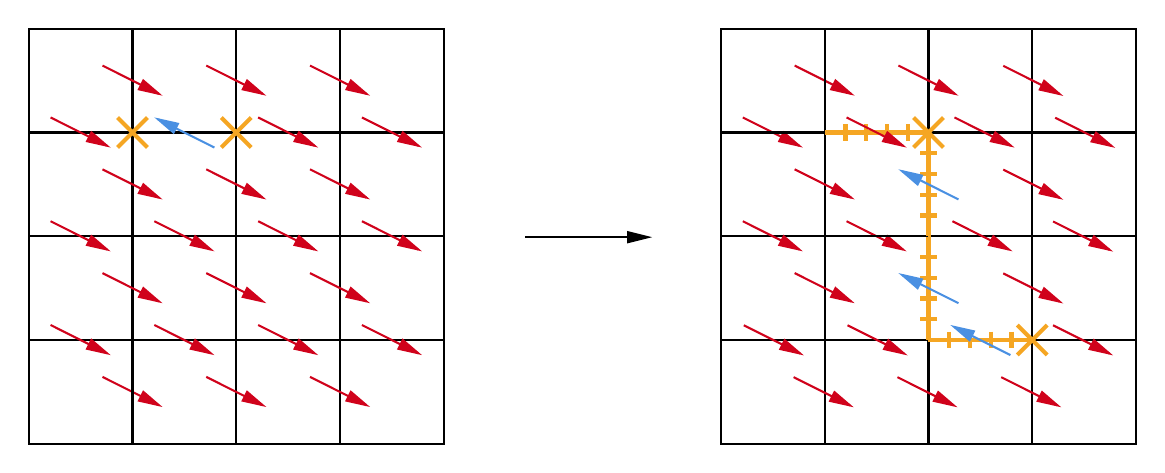
\begin{tikzpicture}[x=0.75pt,y=0.75pt,yscale=-1,xscale=1]
%uncomment if require: \path (0,300); %set diagram left start at 0, and has height of 300

%Shape: Square [id:dp36196949269788203] 
\draw   (433,212.06) -- (483,212.06) -- (483,262.06) -- (433,262.06) -- cycle ;
%Shape: Square [id:dp4539886973873315] 
\draw   (533,212.06) -- (583,212.06) -- (583,262.06) -- (533,262.06) -- cycle ;
%Shape: Square [id:dp6375978130473219] 
\draw   (533,162.06) -- (583,162.06) -- (583,212.06) -- (533,212.06) -- cycle ;
%Shape: Square [id:dp5485656687226403] 
\draw   (483,212.06) -- (533,212.06) -- (533,262.06) -- (483,262.06) -- cycle ;
%Shape: Square [id:dp7861946257195895] 
\draw   (383,62.06) -- (433,62.06) -- (433,112.06) -- (383,112.06) -- cycle ;
%Shape: Square [id:dp4265689791603251] 
\draw   (433,62.06) -- (483,62.06) -- (483,112.06) -- (433,112.06) -- cycle ;
%Shape: Square [id:dp85770876091055] 
\draw   (383,112.06) -- (433,112.06) -- (433,162.06) -- (383,162.06) -- cycle ;
%Shape: Square [id:dp9994589809447718] 
\draw   (433,112.06) -- (483,112.06) -- (483,162.06) -- (433,162.06) -- cycle ;
%Shape: Square [id:dp3934144084207285] 
\draw   (483,62.06) -- (533,62.06) -- (533,112.06) -- (483,112.06) -- cycle ;
%Shape: Square [id:dp44660161866059256] 
\draw   (483,112.06) -- (533,112.06) -- (533,162.06) -- (483,162.06) -- cycle ;
%Shape: Square [id:dp8655676597107462] 
\draw   (383,162.06) -- (433,162.06) -- (433,212.06) -- (383,212.06) -- cycle ;
%Shape: Square [id:dp31081007435708097] 
\draw   (433,162.06) -- (483,162.06) -- (483,212.06) -- (433,212.06) -- cycle ;
%Shape: Square [id:dp8086659149268767] 
\draw   (483,162.06) -- (533,162.06) -- (533,212.06) -- (483,212.06) -- cycle ;
%Straight Lines [id:da053200549000906205] 
\draw [color={rgb, 255:red, 245; green, 166; blue, 35 }  ,draw opacity=1 ][line width=1.5]    (533,212.06) ;
\draw [shift={(533,212.06)}, rotate = 45] [color={rgb, 255:red, 245; green, 166; blue, 35 }  ,draw opacity=1 ][line width=1.5]    (-10.17,0) -- (10.17,0)(0,10.17) -- (0,-10.17)   ;
%Straight Lines [id:da3649892359785114] 
\draw [color={rgb, 255:red, 245; green, 166; blue, 35 }  ,draw opacity=1 ][line width=1.5]    (483,212.06) -- (533,212.06) (493,208.06) -- (493,216.06)(503,208.06) -- (503,216.06)(513,208.06) -- (513,216.06)(523,208.06) -- (523,216.06) ;
%Straight Lines [id:da13469057648466287] 
\draw [color={rgb, 255:red, 245; green, 166; blue, 35 }  ,draw opacity=1 ][line width=1.5]    (483,212.06) -- (483,162.06) (479,202.06) -- (487,202.06)(479,192.06) -- (487,192.06)(479,182.06) -- (487,182.06)(479,172.06) -- (487,172.06) ;
%Straight Lines [id:da6345763045380002] 
\draw [color={rgb, 255:red, 208; green, 2; blue, 27 }  ,draw opacity=1 ]   (418.54,79.81) -- (445.67,93.42) ;
\draw [shift={(447.46,94.31)}, rotate = 206.63] [fill={rgb, 255:red, 208; green, 2; blue, 27 }  ,fill opacity=1 ][line width=0.08]  [draw opacity=0] (12,-3) -- (0,0) -- (12,3) -- cycle    ;
%Straight Lines [id:da5007686616056861] 
\draw    (433,62.06) -- (433,112.06) ;
%Straight Lines [id:da49682550012597915] 
\draw    (433,112.06) -- (433,162.06) ;
%Straight Lines [id:da9160145620735776] 
\draw [color={rgb, 255:red, 208; green, 2; blue, 27 }  ,draw opacity=1 ]   (393.54,104.81) -- (420.67,118.42) ;
\draw [shift={(422.46,119.31)}, rotate = 206.63] [fill={rgb, 255:red, 208; green, 2; blue, 27 }  ,fill opacity=1 ][line width=0.08]  [draw opacity=0] (12,-3) -- (0,0) -- (12,3) -- cycle    ;
%Straight Lines [id:da6394802587540938] 
\draw    (383,112.06) -- (433,112.06) ;
%Straight Lines [id:da32113469950640705] 
\draw [color={rgb, 255:red, 208; green, 2; blue, 27 }  ,draw opacity=1 ]   (418.54,129.81) -- (445.67,143.42) ;
\draw [shift={(447.46,144.31)}, rotate = 206.63] [fill={rgb, 255:red, 208; green, 2; blue, 27 }  ,fill opacity=1 ][line width=0.08]  [draw opacity=0] (12,-3) -- (0,0) -- (12,3) -- cycle    ;
%Straight Lines [id:da24099776716939703] 
\draw [color={rgb, 255:red, 74; green, 144; blue, 226 }  ,draw opacity=1 ]   (497.46,194.31) -- (470.33,180.71) ;
\draw [shift={(468.54,179.81)}, rotate = 386.63] [fill={rgb, 255:red, 74; green, 144; blue, 226 }  ,fill opacity=1 ][line width=0.08]  [draw opacity=0] (12,-3) -- (0,0) -- (12,3) -- cycle    ;
%Straight Lines [id:da5688629141790045] 
\draw [color={rgb, 255:red, 74; green, 144; blue, 226 }  ,draw opacity=1 ]   (522.46,219.31) -- (495.33,205.71) ;
\draw [shift={(493.54,204.81)}, rotate = 386.63] [fill={rgb, 255:red, 74; green, 144; blue, 226 }  ,fill opacity=1 ][line width=0.08]  [draw opacity=0] (12,-3) -- (0,0) -- (12,3) -- cycle    ;
%Straight Lines [id:da06719454989257079] 
\draw    (483,62.06) -- (483,112.06) ;
%Straight Lines [id:da3658940630124152] 
\draw [color={rgb, 255:red, 208; green, 2; blue, 27 }  ,draw opacity=1 ]   (468.54,79.81) -- (495.67,93.42) ;
\draw [shift={(497.46,94.31)}, rotate = 206.63] [fill={rgb, 255:red, 208; green, 2; blue, 27 }  ,fill opacity=1 ][line width=0.08]  [draw opacity=0] (12,-3) -- (0,0) -- (12,3) -- cycle    ;
%Straight Lines [id:da9827136653687769] 
\draw [color={rgb, 255:red, 208; green, 2; blue, 27 }  ,draw opacity=1 ]   (443.54,154.81) -- (470.67,168.42) ;
\draw [shift={(472.46,169.31)}, rotate = 206.63] [fill={rgb, 255:red, 208; green, 2; blue, 27 }  ,fill opacity=1 ][line width=0.08]  [draw opacity=0] (12,-3) -- (0,0) -- (12,3) -- cycle    ;
%Straight Lines [id:da24542517630533744] 
\draw    (433,162.06) -- (483,162.06) ;
%Straight Lines [id:da675706435803094] 
\draw [color={rgb, 255:red, 245; green, 166; blue, 35 }  ,draw opacity=1 ][line width=1.5]    (433,112.06) -- (483,112.06) (443,108.06) -- (443,116.06)(453,108.06) -- (453,116.06)(463,108.06) -- (463,116.06)(473,108.06) -- (473,116.06) ;
%Straight Lines [id:da7807078761743926] 
\draw [color={rgb, 255:red, 245; green, 166; blue, 35 }  ,draw opacity=1 ][line width=1.5]    (483,162.06) -- (483,112.06) (479,152.06) -- (487,152.06)(479,142.06) -- (487,142.06)(479,132.06) -- (487,132.06)(479,122.06) -- (487,122.06) ;
%Straight Lines [id:da49273110414826204] 
\draw    (383,162.06) -- (433,162.06) ;
%Straight Lines [id:da4909188469525809] 
\draw [color={rgb, 255:red, 208; green, 2; blue, 27 }  ,draw opacity=1 ]   (393.54,154.81) -- (420.67,168.42) ;
\draw [shift={(422.46,169.31)}, rotate = 206.63] [fill={rgb, 255:red, 208; green, 2; blue, 27 }  ,fill opacity=1 ][line width=0.08]  [draw opacity=0] (12,-3) -- (0,0) -- (12,3) -- cycle    ;
%Straight Lines [id:da7732976407163501] 
\draw    (433,162.06) -- (433,212.06) ;
%Straight Lines [id:da8885840601877579] 
\draw [color={rgb, 255:red, 208; green, 2; blue, 27 }  ,draw opacity=1 ]   (418.54,179.81) -- (445.67,193.42) ;
\draw [shift={(447.46,194.31)}, rotate = 206.63] [fill={rgb, 255:red, 208; green, 2; blue, 27 }  ,fill opacity=1 ][line width=0.08]  [draw opacity=0] (12,-3) -- (0,0) -- (12,3) -- cycle    ;
%Straight Lines [id:da7563618305941129] 
\draw [color={rgb, 255:red, 208; green, 2; blue, 27 }  ,draw opacity=1 ]   (494.54,154.81) -- (521.67,168.42) ;
\draw [shift={(523.46,169.31)}, rotate = 206.63] [fill={rgb, 255:red, 208; green, 2; blue, 27 }  ,fill opacity=1 ][line width=0.08]  [draw opacity=0] (12,-3) -- (0,0) -- (12,3) -- cycle    ;
%Straight Lines [id:da8614606849485955] 
\draw [color={rgb, 255:red, 208; green, 2; blue, 27 }  ,draw opacity=1 ]   (495.54,104.81) -- (522.67,118.42) ;
\draw [shift={(524.46,119.31)}, rotate = 206.63] [fill={rgb, 255:red, 208; green, 2; blue, 27 }  ,fill opacity=1 ][line width=0.08]  [draw opacity=0] (12,-3) -- (0,0) -- (12,3) -- cycle    ;
%Straight Lines [id:da7939198814652852] 
\draw [color={rgb, 255:red, 74; green, 144; blue, 226 }  ,draw opacity=1 ]   (497.46,144.31) -- (470.33,130.71) ;
\draw [shift={(468.54,129.81)}, rotate = 386.63] [fill={rgb, 255:red, 74; green, 144; blue, 226 }  ,fill opacity=1 ][line width=0.08]  [draw opacity=0] (12,-3) -- (0,0) -- (12,3) -- cycle    ;
%Shape: Square [id:dp106338857848296] 
\draw   (383,212.06) -- (433,212.06) -- (433,262.06) -- (383,262.06) -- cycle ;
%Shape: Square [id:dp707576745510903] 
\draw   (533,62.06) -- (583,62.06) -- (583,112.06) -- (533,112.06) -- cycle ;
%Shape: Square [id:dp32996281885734047] 
\draw   (533,112.06) -- (583,112.06) -- (583,162.06) -- (533,162.06) -- cycle ;
%Straight Lines [id:da9598175384692527] 
\draw [color={rgb, 255:red, 208; green, 2; blue, 27 }  ,draw opacity=1 ]   (518.04,229.94) -- (545.17,243.54) ;
\draw [shift={(546.96,244.44)}, rotate = 206.63] [fill={rgb, 255:red, 208; green, 2; blue, 27 }  ,fill opacity=1 ][line width=0.08]  [draw opacity=0] (12,-3) -- (0,0) -- (12,3) -- cycle    ;
%Straight Lines [id:da830133254314485] 
\draw [color={rgb, 255:red, 208; green, 2; blue, 27 }  ,draw opacity=1 ]   (468.04,229.94) -- (495.17,243.54) ;
\draw [shift={(496.96,244.44)}, rotate = 206.63] [fill={rgb, 255:red, 208; green, 2; blue, 27 }  ,fill opacity=1 ][line width=0.08]  [draw opacity=0] (12,-3) -- (0,0) -- (12,3) -- cycle    ;
%Straight Lines [id:da9456594973520096] 
\draw [color={rgb, 255:red, 208; green, 2; blue, 27 }  ,draw opacity=1 ]   (418.04,229.94) -- (445.17,243.54) ;
\draw [shift={(446.96,244.44)}, rotate = 206.63] [fill={rgb, 255:red, 208; green, 2; blue, 27 }  ,fill opacity=1 ][line width=0.08]  [draw opacity=0] (12,-3) -- (0,0) -- (12,3) -- cycle    ;
%Straight Lines [id:da9286370031442577] 
\draw    (532.5,112.19) -- (582.5,112.19) ;
%Straight Lines [id:da05035735074794423] 
\draw [color={rgb, 255:red, 208; green, 2; blue, 27 }  ,draw opacity=1 ]   (543.04,154.94) -- (570.17,168.54) ;
\draw [shift={(571.96,169.44)}, rotate = 206.63] [fill={rgb, 255:red, 208; green, 2; blue, 27 }  ,fill opacity=1 ][line width=0.08]  [draw opacity=0] (12,-3) -- (0,0) -- (12,3) -- cycle    ;
%Straight Lines [id:da3083548171838988] 
\draw [color={rgb, 255:red, 208; green, 2; blue, 27 }  ,draw opacity=1 ]   (543.04,204.94) -- (570.17,218.54) ;
\draw [shift={(571.96,219.44)}, rotate = 206.63] [fill={rgb, 255:red, 208; green, 2; blue, 27 }  ,fill opacity=1 ][line width=0.08]  [draw opacity=0] (12,-3) -- (0,0) -- (12,3) -- cycle    ;
%Straight Lines [id:da8166890828993534] 
\draw [color={rgb, 255:red, 208; green, 2; blue, 27 }  ,draw opacity=1 ]   (394.04,204.94) -- (421.17,218.54) ;
\draw [shift={(422.96,219.44)}, rotate = 206.63] [fill={rgb, 255:red, 208; green, 2; blue, 27 }  ,fill opacity=1 ][line width=0.08]  [draw opacity=0] (12,-3) -- (0,0) -- (12,3) -- cycle    ;
%Straight Lines [id:da8554659211608935] 
\draw [color={rgb, 255:red, 208; green, 2; blue, 27 }  ,draw opacity=1 ]   (544.04,104.94) -- (571.17,118.54) ;
\draw [shift={(572.96,119.44)}, rotate = 206.63] [fill={rgb, 255:red, 208; green, 2; blue, 27 }  ,fill opacity=1 ][line width=0.08]  [draw opacity=0] (12,-3) -- (0,0) -- (12,3) -- cycle    ;
%Straight Lines [id:da5375248801254273] 
\draw [color={rgb, 255:red, 208; green, 2; blue, 27 }  ,draw opacity=1 ]   (444.04,204.94) -- (471.17,218.54) ;
\draw [shift={(472.96,219.44)}, rotate = 206.63] [fill={rgb, 255:red, 208; green, 2; blue, 27 }  ,fill opacity=1 ][line width=0.08]  [draw opacity=0] (12,-3) -- (0,0) -- (12,3) -- cycle    ;
%Straight Lines [id:da09821728349202297] 
\draw [color={rgb, 255:red, 208; green, 2; blue, 27 }  ,draw opacity=1 ]   (519.04,129.94) -- (546.17,143.54) ;
\draw [shift={(547.96,144.44)}, rotate = 206.63] [fill={rgb, 255:red, 208; green, 2; blue, 27 }  ,fill opacity=1 ][line width=0.08]  [draw opacity=0] (12,-3) -- (0,0) -- (12,3) -- cycle    ;
%Straight Lines [id:da9512899383990645] 
\draw [color={rgb, 255:red, 208; green, 2; blue, 27 }  ,draw opacity=1 ]   (519.04,179.94) -- (546.17,193.54) ;
\draw [shift={(547.96,194.44)}, rotate = 206.63] [fill={rgb, 255:red, 208; green, 2; blue, 27 }  ,fill opacity=1 ][line width=0.08]  [draw opacity=0] (12,-3) -- (0,0) -- (12,3) -- cycle    ;
%Straight Lines [id:da535357998535275] 
\draw [color={rgb, 255:red, 208; green, 2; blue, 27 }  ,draw opacity=1 ]   (519.04,79.94) -- (546.17,93.54) ;
\draw [shift={(547.96,94.44)}, rotate = 206.63] [fill={rgb, 255:red, 208; green, 2; blue, 27 }  ,fill opacity=1 ][line width=0.08]  [draw opacity=0] (12,-3) -- (0,0) -- (12,3) -- cycle    ;
%Shape: Square [id:dp7990222049361821] 
\draw   (49.5,62.06) -- (99.5,62.06) -- (99.5,112.06) -- (49.5,112.06) -- cycle ;
%Shape: Square [id:dp8904550552386634] 
\draw   (99.5,62.06) -- (149.5,62.06) -- (149.5,112.06) -- (99.5,112.06) -- cycle ;
%Shape: Square [id:dp5127650109295845] 
\draw   (49.5,112.06) -- (99.5,112.06) -- (99.5,162.06) -- (49.5,162.06) -- cycle ;
%Shape: Square [id:dp12849214688436494] 
\draw   (99.5,112.06) -- (149.5,112.06) -- (149.5,162.06) -- (99.5,162.06) -- cycle ;
%Shape: Square [id:dp7737277027683318] 
\draw   (149.5,62.06) -- (199.5,62.06) -- (199.5,112.06) -- (149.5,112.06) -- cycle ;
%Shape: Square [id:dp7927352395037797] 
\draw   (149.5,112.06) -- (199.5,112.06) -- (199.5,162.06) -- (149.5,162.06) -- cycle ;
%Shape: Square [id:dp5386554622216682] 
\draw   (49.5,162.06) -- (99.5,162.06) -- (99.5,212.06) -- (49.5,212.06) -- cycle ;
%Shape: Square [id:dp111010476712055] 
\draw   (99.5,162.06) -- (149.5,162.06) -- (149.5,212.06) -- (99.5,212.06) -- cycle ;
%Shape: Square [id:dp5821419956800287] 
\draw   (149.5,162.06) -- (199.5,162.06) -- (199.5,212.06) -- (149.5,212.06) -- cycle ;
%Straight Lines [id:da6903696329395099] 
\draw    (99.5,62.06) -- (99.5,112.06) ;
%Straight Lines [id:da37681750055959395] 
\draw    (99.5,112.06) -- (99.5,162.06) ;
%Straight Lines [id:da07589525156843258] 
\draw    (49.5,112.06) -- (99.5,112.06) ;
%Straight Lines [id:da8308006113905104] 
\draw    (149.5,62.06) -- (149.5,112.06) ;
%Straight Lines [id:da7674707191655699] 
\draw    (99.5,162.06) -- (149.5,162.06) ;
%Straight Lines [id:da7594879654833071] 
\draw    (49.5,162.06) -- (99.5,162.06) ;
%Straight Lines [id:da027284503407192018] 
\draw    (99.5,162.06) -- (99.5,212.06) ;
%Straight Lines [id:da4901240737698671] 
\draw [color={rgb, 255:red, 208; green, 2; blue, 27 }  ,draw opacity=1 ]   (85.04,79.81) -- (112.17,93.42) ;
\draw [shift={(113.96,94.31)}, rotate = 206.63] [fill={rgb, 255:red, 208; green, 2; blue, 27 }  ,fill opacity=1 ][line width=0.08]  [draw opacity=0] (12,-3) -- (0,0) -- (12,3) -- cycle    ;
%Straight Lines [id:da6150555493961845] 
\draw    (149.5,112.06) -- (149.5,162.06) ;
%Straight Lines [id:da8116460068940423] 
\draw    (149.5,162.06) -- (149.5,212.06) ;
%Straight Lines [id:da5488283476959541] 
\draw    (149.5,112.06) -- (199.5,112.06) ;
%Straight Lines [id:da07732657367073692] 
\draw    (149.5,162.06) -- (199.5,162.06) ;
%Straight Lines [id:da28030930112021957] 
\draw    (99.5,112.06) -- (149.5,112.06) ;
%Straight Lines [id:da033793134933984836] 
\draw [color={rgb, 255:red, 208; green, 2; blue, 27 }  ,draw opacity=1 ]   (135.04,79.81) -- (162.17,93.42) ;
\draw [shift={(163.96,94.31)}, rotate = 206.63] [fill={rgb, 255:red, 208; green, 2; blue, 27 }  ,fill opacity=1 ][line width=0.08]  [draw opacity=0] (12,-3) -- (0,0) -- (12,3) -- cycle    ;
%Straight Lines [id:da8814413169220066] 
\draw [color={rgb, 255:red, 208; green, 2; blue, 27 }  ,draw opacity=1 ]   (443.54,104.81) -- (470.67,118.42) ;
\draw [shift={(472.46,119.31)}, rotate = 206.63] [fill={rgb, 255:red, 208; green, 2; blue, 27 }  ,fill opacity=1 ][line width=0.08]  [draw opacity=0] (12,-3) -- (0,0) -- (12,3) -- cycle    ;
%Straight Lines [id:da7806079605744642] 
\draw [color={rgb, 255:red, 208; green, 2; blue, 27 }  ,draw opacity=1 ]   (60.04,104.81) -- (87.17,118.42) ;
\draw [shift={(88.96,119.31)}, rotate = 206.63] [fill={rgb, 255:red, 208; green, 2; blue, 27 }  ,fill opacity=1 ][line width=0.08]  [draw opacity=0] (12,-3) -- (0,0) -- (12,3) -- cycle    ;
%Straight Lines [id:da5754931816488336] 
\draw [color={rgb, 255:red, 208; green, 2; blue, 27 }  ,draw opacity=1 ]   (160.04,104.81) -- (187.17,118.42) ;
\draw [shift={(188.96,119.31)}, rotate = 206.63] [fill={rgb, 255:red, 208; green, 2; blue, 27 }  ,fill opacity=1 ][line width=0.08]  [draw opacity=0] (12,-3) -- (0,0) -- (12,3) -- cycle    ;
%Straight Lines [id:da5952100515604342] 
\draw [color={rgb, 255:red, 208; green, 2; blue, 27 }  ,draw opacity=1 ]   (85.04,129.81) -- (112.17,143.42) ;
\draw [shift={(113.96,144.31)}, rotate = 206.63] [fill={rgb, 255:red, 208; green, 2; blue, 27 }  ,fill opacity=1 ][line width=0.08]  [draw opacity=0] (12,-3) -- (0,0) -- (12,3) -- cycle    ;
%Straight Lines [id:da9410359840468674] 
\draw [color={rgb, 255:red, 208; green, 2; blue, 27 }  ,draw opacity=1 ]   (135.04,129.81) -- (162.17,143.42) ;
\draw [shift={(163.96,144.31)}, rotate = 206.63] [fill={rgb, 255:red, 208; green, 2; blue, 27 }  ,fill opacity=1 ][line width=0.08]  [draw opacity=0] (12,-3) -- (0,0) -- (12,3) -- cycle    ;
%Straight Lines [id:da18562201002496082] 
\draw [color={rgb, 255:red, 208; green, 2; blue, 27 }  ,draw opacity=1 ]   (110.04,154.81) -- (137.17,168.42) ;
\draw [shift={(138.96,169.31)}, rotate = 206.63] [fill={rgb, 255:red, 208; green, 2; blue, 27 }  ,fill opacity=1 ][line width=0.08]  [draw opacity=0] (12,-3) -- (0,0) -- (12,3) -- cycle    ;
%Straight Lines [id:da11755833098770019] 
\draw [color={rgb, 255:red, 208; green, 2; blue, 27 }  ,draw opacity=1 ]   (160.04,154.81) -- (187.17,168.42) ;
\draw [shift={(188.96,169.31)}, rotate = 206.63] [fill={rgb, 255:red, 208; green, 2; blue, 27 }  ,fill opacity=1 ][line width=0.08]  [draw opacity=0] (12,-3) -- (0,0) -- (12,3) -- cycle    ;
%Straight Lines [id:da25442080979156234] 
\draw [color={rgb, 255:red, 208; green, 2; blue, 27 }  ,draw opacity=1 ]   (60.04,154.81) -- (87.17,168.42) ;
\draw [shift={(88.96,169.31)}, rotate = 206.63] [fill={rgb, 255:red, 208; green, 2; blue, 27 }  ,fill opacity=1 ][line width=0.08]  [draw opacity=0] (12,-3) -- (0,0) -- (12,3) -- cycle    ;
%Straight Lines [id:da44143500096146715] 
\draw [color={rgb, 255:red, 208; green, 2; blue, 27 }  ,draw opacity=1 ]   (85.04,179.81) -- (112.17,193.42) ;
\draw [shift={(113.96,194.31)}, rotate = 206.63] [fill={rgb, 255:red, 208; green, 2; blue, 27 }  ,fill opacity=1 ][line width=0.08]  [draw opacity=0] (12,-3) -- (0,0) -- (12,3) -- cycle    ;
%Straight Lines [id:da6699778566324532] 
\draw [color={rgb, 255:red, 208; green, 2; blue, 27 }  ,draw opacity=1 ]   (135.04,179.81) -- (162.17,193.42) ;
\draw [shift={(163.96,194.31)}, rotate = 206.63] [fill={rgb, 255:red, 208; green, 2; blue, 27 }  ,fill opacity=1 ][line width=0.08]  [draw opacity=0] (12,-3) -- (0,0) -- (12,3) -- cycle    ;
%Straight Lines [id:da9200325240479144] 
\draw    (199.5,62.06) -- (199.5,112.06) ;
%Shape: Square [id:dp7328942993667524] 
\draw   (199.5,112.06) -- (249.5,112.06) -- (249.5,162.06) -- (199.5,162.06) -- cycle ;
%Shape: Square [id:dp2890961291771639] 
\draw   (199.5,162.06) -- (249.5,162.06) -- (249.5,212.06) -- (199.5,212.06) -- cycle ;
%Shape: Square [id:dp2899655977518478] 
\draw   (199.5,62.06) -- (249.5,62.06) -- (249.5,112.06) -- (199.5,112.06) -- cycle ;
%Shape: Square [id:dp04410279330347566] 
\draw   (49.5,212.06) -- (99.5,212.06) -- (99.5,262.06) -- (49.5,262.06) -- cycle ;
%Shape: Square [id:dp4328001959850347] 
\draw   (99.5,212.06) -- (149.5,212.06) -- (149.5,262.06) -- (99.5,262.06) -- cycle ;
%Shape: Square [id:dp9817380452635807] 
\draw   (149.5,212.06) -- (199.5,212.06) -- (199.5,262.06) -- (149.5,262.06) -- cycle ;
%Shape: Square [id:dp6981091681806493] 
\draw   (199.5,212.06) -- (249.5,212.06) -- (249.5,262.06) -- (199.5,262.06) -- cycle ;
%Straight Lines [id:da5538961608697273] 
\draw [color={rgb, 255:red, 208; green, 2; blue, 27 }  ,draw opacity=1 ]   (185.04,79.81) -- (212.17,93.42) ;
\draw [shift={(213.96,94.31)}, rotate = 206.63] [fill={rgb, 255:red, 208; green, 2; blue, 27 }  ,fill opacity=1 ][line width=0.08]  [draw opacity=0] (12,-3) -- (0,0) -- (12,3) -- cycle    ;
%Straight Lines [id:da8078206711036395] 
\draw    (199.5,112.06) -- (199.5,162.06) ;
%Straight Lines [id:da23005360080717563] 
\draw    (199.5,162.06) -- (199.5,212.06) ;
%Straight Lines [id:da7962686121202824] 
\draw    (199.5,212.06) -- (199.5,262.06) ;
%Straight Lines [id:da9889990147566594] 
\draw    (149.5,212.06) -- (149.5,262.06) ;
%Straight Lines [id:da7694764072279323] 
\draw    (99.5,212.06) -- (99.5,262.06) ;
%Straight Lines [id:da2376018785872358] 
\draw [color={rgb, 255:red, 208; green, 2; blue, 27 }  ,draw opacity=1 ]   (185.04,129.81) -- (212.17,143.42) ;
\draw [shift={(213.96,144.31)}, rotate = 206.63] [fill={rgb, 255:red, 208; green, 2; blue, 27 }  ,fill opacity=1 ][line width=0.08]  [draw opacity=0] (12,-3) -- (0,0) -- (12,3) -- cycle    ;
%Straight Lines [id:da5207260238843008] 
\draw [color={rgb, 255:red, 208; green, 2; blue, 27 }  ,draw opacity=1 ]   (185.04,179.81) -- (212.17,193.42) ;
\draw [shift={(213.96,194.31)}, rotate = 206.63] [fill={rgb, 255:red, 208; green, 2; blue, 27 }  ,fill opacity=1 ][line width=0.08]  [draw opacity=0] (12,-3) -- (0,0) -- (12,3) -- cycle    ;
%Straight Lines [id:da5480042946717876] 
\draw [color={rgb, 255:red, 208; green, 2; blue, 27 }  ,draw opacity=1 ]   (185.04,229.81) -- (212.17,243.42) ;
\draw [shift={(213.96,244.31)}, rotate = 206.63] [fill={rgb, 255:red, 208; green, 2; blue, 27 }  ,fill opacity=1 ][line width=0.08]  [draw opacity=0] (12,-3) -- (0,0) -- (12,3) -- cycle    ;
%Straight Lines [id:da5023843690724528] 
\draw [color={rgb, 255:red, 208; green, 2; blue, 27 }  ,draw opacity=1 ]   (135.04,229.81) -- (162.17,243.42) ;
\draw [shift={(163.96,244.31)}, rotate = 206.63] [fill={rgb, 255:red, 208; green, 2; blue, 27 }  ,fill opacity=1 ][line width=0.08]  [draw opacity=0] (12,-3) -- (0,0) -- (12,3) -- cycle    ;
%Straight Lines [id:da48659723265136146] 
\draw [color={rgb, 255:red, 208; green, 2; blue, 27 }  ,draw opacity=1 ]   (85.04,229.81) -- (112.17,243.42) ;
\draw [shift={(113.96,244.31)}, rotate = 206.63] [fill={rgb, 255:red, 208; green, 2; blue, 27 }  ,fill opacity=1 ][line width=0.08]  [draw opacity=0] (12,-3) -- (0,0) -- (12,3) -- cycle    ;
%Straight Lines [id:da08436190038107028] 
\draw    (99.5,212.06) -- (99.5,262.06) ;
%Straight Lines [id:da8238882701325334] 
\draw    (49.5,212.06) -- (99.5,212.06) ;
%Straight Lines [id:da4713034331032184] 
\draw    (199.5,112.06) -- (249.5,112.06) ;
%Straight Lines [id:da06868085071667629] 
\draw    (199.5,162.06) -- (249.5,162.06) ;
%Straight Lines [id:da5820074071163888] 
\draw    (199.5,212.06) -- (249.5,212.06) ;
%Straight Lines [id:da44314860743375517] 
\draw [color={rgb, 255:red, 208; green, 2; blue, 27 }  ,draw opacity=1 ]   (60.04,204.81) -- (87.17,218.42) ;
\draw [shift={(88.96,219.31)}, rotate = 206.63] [fill={rgb, 255:red, 208; green, 2; blue, 27 }  ,fill opacity=1 ][line width=0.08]  [draw opacity=0] (12,-3) -- (0,0) -- (12,3) -- cycle    ;
%Straight Lines [id:da059395541772979454] 
\draw [color={rgb, 255:red, 208; green, 2; blue, 27 }  ,draw opacity=1 ]   (210.04,104.81) -- (237.17,118.42) ;
\draw [shift={(238.96,119.31)}, rotate = 206.63] [fill={rgb, 255:red, 208; green, 2; blue, 27 }  ,fill opacity=1 ][line width=0.08]  [draw opacity=0] (12,-3) -- (0,0) -- (12,3) -- cycle    ;
%Straight Lines [id:da5063118933962647] 
\draw [color={rgb, 255:red, 208; green, 2; blue, 27 }  ,draw opacity=1 ]   (210.04,154.81) -- (237.17,168.42) ;
\draw [shift={(238.96,169.31)}, rotate = 206.63] [fill={rgb, 255:red, 208; green, 2; blue, 27 }  ,fill opacity=1 ][line width=0.08]  [draw opacity=0] (12,-3) -- (0,0) -- (12,3) -- cycle    ;
%Straight Lines [id:da3889893206026507] 
\draw [color={rgb, 255:red, 208; green, 2; blue, 27 }  ,draw opacity=1 ]   (210.04,204.81) -- (237.17,218.42) ;
\draw [shift={(238.96,219.31)}, rotate = 206.63] [fill={rgb, 255:red, 208; green, 2; blue, 27 }  ,fill opacity=1 ][line width=0.08]  [draw opacity=0] (12,-3) -- (0,0) -- (12,3) -- cycle    ;
%Straight Lines [id:da643594178741393] 
\draw    (99.5,212.06) -- (149.5,212.06) ;
%Straight Lines [id:da8957855859845023] 
\draw    (149.5,212.06) -- (199.5,212.06) ;
%Straight Lines [id:da6024482081021001] 
\draw [color={rgb, 255:red, 208; green, 2; blue, 27 }  ,draw opacity=1 ]   (160.04,204.81) -- (187.17,218.42) ;
\draw [shift={(188.96,219.31)}, rotate = 206.63] [fill={rgb, 255:red, 208; green, 2; blue, 27 }  ,fill opacity=1 ][line width=0.08]  [draw opacity=0] (12,-3) -- (0,0) -- (12,3) -- cycle    ;
%Straight Lines [id:da25598314352120677] 
\draw [color={rgb, 255:red, 208; green, 2; blue, 27 }  ,draw opacity=1 ]   (110.04,204.81) -- (137.17,218.42) ;
\draw [shift={(138.96,219.31)}, rotate = 206.63] [fill={rgb, 255:red, 208; green, 2; blue, 27 }  ,fill opacity=1 ][line width=0.08]  [draw opacity=0] (12,-3) -- (0,0) -- (12,3) -- cycle    ;
%Straight Lines [id:da6536230781419683] 
\draw    (288.83,162.5) -- (347.83,162.5) ;
\draw [shift={(349.83,162.5)}, rotate = 180] [fill={rgb, 255:red, 0; green, 0; blue, 0 }  ][line width=0.08]  [draw opacity=0] (12,-3) -- (0,0) -- (12,3) -- cycle    ;
%Straight Lines [id:da9507304761845745] 
\draw [color={rgb, 255:red, 74; green, 144; blue, 226 }  ,draw opacity=1 ]   (138.96,119.31) -- (111.83,105.71) ;
\draw [shift={(110.04,104.81)}, rotate = 386.63] [fill={rgb, 255:red, 74; green, 144; blue, 226 }  ,fill opacity=1 ][line width=0.08]  [draw opacity=0] (12,-3) -- (0,0) -- (12,3) -- cycle    ;
%Straight Lines [id:da5344654488798346] 
\draw [color={rgb, 255:red, 245; green, 166; blue, 35 }  ,draw opacity=1 ][line width=1.5]    (99.5,112.06) ;
\draw [shift={(99.5,112.06)}, rotate = 45] [color={rgb, 255:red, 245; green, 166; blue, 35 }  ,draw opacity=1 ][line width=1.5]    (-10.17,0) -- (10.17,0)(0,10.17) -- (0,-10.17)   ;
%Straight Lines [id:da7415055109194719] 
\draw [color={rgb, 255:red, 245; green, 166; blue, 35 }  ,draw opacity=1 ][line width=1.5]    (149.5,112.06) ;
\draw [shift={(149.5,112.06)}, rotate = 45] [color={rgb, 255:red, 245; green, 166; blue, 35 }  ,draw opacity=1 ][line width=1.5]    (-10.17,0) -- (10.17,0)(0,10.17) -- (0,-10.17)   ;
%Straight Lines [id:da6351670278271098] 
\draw [color={rgb, 255:red, 245; green, 166; blue, 35 }  ,draw opacity=1 ][line width=1.5]    (483,112.06) ;
\draw [shift={(483,112.06)}, rotate = 45] [color={rgb, 255:red, 245; green, 166; blue, 35 }  ,draw opacity=1 ][line width=1.5]    (-10.17,0) -- (10.17,0)(0,10.17) -- (0,-10.17)   ;




\end{tikzpicture}

    }
    \caption{Toric-code模型的$O_\text{e}$开弦算符}
\end{figure}

两种激发成对出现的事实意味着可以使用弦算符描述它们的产生和消灭。%
\footnote{
    一个可能的疑难是,当任意子交换产生的相位差非常小,接近$0$和$\pi$时,系统应该平滑地过渡到玻色子系统或者费米子系统上,但是费米子系统和玻色子系统可以使用局域的场算符描述,似乎并没有方法能够平滑地从弦算符过渡到场算符上。
    这里的答案是,有一些定理保证了有限个任意子交换后产生的相位差是代数数,从而不能够连续地调节相位差。
    因此任意子和玻色子、费米子之间是不能够平滑地过渡的。

    任意子激发是弦算符产生的,我们可以追踪每个任意子的位置,或者按照量子场论的套路,我们似乎应该讨论弦算符的动力学。不过应当注意,由于很多弦算符(如闭弦)本身并不增加或者减少系统能量,我们实际上不需要一般的关于弦的理论,一定有一些更加平凡的理论——通常是某个拓扑量子场论——等价于任意子模型。
    例如,一些阿贝尔拓扑序可以使用Chern-Simons理论描述。
}%
首先考虑由一条边连接的两个格点,这条边上的${\sigma}^z_{\vb*{i}}$算符可以将这条边上的$x$方向的自旋翻转,因此它可以做到以下三件事:
\begin{itemize}
    \item 如果两个格点上原本没有e粒子,那么在两个格点上同时产生e粒子;
    \item 如果两个格点上原本都有e粒子,那么在两个格点上同时消灭e粒子; 
    \item 如果两个格点一个有e粒子一个没有,那么该e粒子将被转移到原本没有e粒子的格点上。
\end{itemize}
这样设一系列首尾相连的边$\{\vb*{l}\}$连接了两个格点,则弦算符
\begin{equation}
    {O}_\text{e} = \prod_{\vb*{l}} {\sigma}_{\vb*{l}}^z
\end{equation}
同样可以做到以上三件事。
同样,将以上论述中的${\sigma}^z$换成${\sigma}^x$,“格点”换成“方块”,“连接两个格点的边”换成“方块共享的边”(我们可以在每个方块中间放置一个点,从而m粒子也定义在一个格点上),同样可以定义弦算符
\begin{equation}
    {O}_\text{m} = \prod_{\vb*{i}} {\sigma}_{\vb*{i}}^x.
\end{equation}
以上讨论的都是开放的弦,闭合的弦的行为需要具体分析,且对闭弦有
\begin{equation}
    {O}_\text{e} \ket{0} = {O}_\text{m} \ket{0} = \ket{0}.
\end{equation}

通过弦算符可以检查e粒子和m粒子绕对方转一圈(实际上就是使用一个闭合的弦算符作用在一个有e粒子或者m粒子的格点上),都会多出来一个$\pi$的相位,这是因为如果一个m粒子闭弦和一个e粒子开弦有单个交点,那么它们反对易(因为同一个边上的${\sigma}^x$和${\sigma}^z$反对易)。
换而言之,e粒子和m粒子均为任意子激发:这是二维的特殊现象,因为二维的环路在二维平面上它围绕的区域被挖掉一个点之后就不可缩了,因此一个粒子转一圈之后可以有一个非零相位变化。
本节涉及的激发尚为阿贝尔统计,即转一圈之后得到的量子态和转之前只差一个$U(1)$变换;还有非阿贝尔统计,即转一圈可以转移到别的量子态上。

\subsection{任意子表}

现在的问题是,环面上的Toric-code模型中最多能够弄出来多少任意子?显然e粒子和m粒子都是任意子,虽然两者自己满足玻色统计,但它们之间有一个非平凡的相位。
我们下面将以拓扑性质分类激发,即,拓扑性质相同的激发算作一种。
可以用两个量来标记一种激发的拓扑性质:设$M_{ab}$为$b$绕着$a$转一圈导致的复数因子,$\theta_a$指的是交换两个$a$导致的复数因子(或者说一个$a$绕着另一个$a$转半圈导致的复数因子)。这样,有
\begin{equation}
    \theta_\mathrm{e} = \theta_\mathrm{m} = 1, \quad M_\mathrm{em} = - 1.
\end{equation}
除了e粒子和m粒子以外肯定还有一种$\mathrm{\epsilon}$粒子,它是一个e粒子和m粒子聚合%
\footnote{所谓聚合指的是将两个激发放得尽可能近,从而得到的复合激发。e粒子和m粒子定义在不同的格点上,因此一个e粒子和一个m粒子的聚合就是在一个正方格子中央放置一个m粒子,在它的某个角上放置一个e粒子之后得到的激发,从远处看这近似于一个粒子。}%
而成的粒子,即
\begin{equation}
    \mathrm{\epsilon} = \mathrm{e} \otimes \mathrm{m}.
\end{equation}
可以容易地验证
\begin{equation}
    M_\mathrm{e\epsilon} = M_\mathrm{m\epsilon} = -1, \quad \theta_\mathrm{\epsilon} = -1.
\end{equation}
e粒子、m粒子和$\mathrm{\epsilon}$粒子这三种拓扑激发都只能成对出现。
除了这三种激发以外还有一些平凡的激发,比如声子之类,将它们全部记为$\mathbbm{1}$。

实际上,e粒子、m粒子和$\epsilon$粒子和$\mathbbm{1}$就是全部拓扑激发。
由于$\mathbbm{1}$无论如何绕圈都不会产生附加的相位,就有
\[
    \mathbbm{1} \otimes a = a.
\]
两个e粒子放在一起,得到的就是某个边上的$\sigma^x$发生了翻转,这是一个普通的激发;m粒子和$\mathrm{\epsilon}$粒子也是如此,于是
\[
    \mathrm{e} \otimes \mathrm{e} = \mathrm{m} \otimes \mathrm{m} = \mathrm{\epsilon} \otimes \mathrm{\epsilon} = \mathbbm{1}.
\]
上式实际上说明了一个非常重要的事实:封闭流形上无论有多少拓扑激发,这个态都可以通过对基态作用一些产生算符得到,或者等价地说改变基态上某些格点的值得到,那么如果将这些拓扑激发聚合到一起,得到的只是基态上局域的一些点被改变了,也即得到了一个平凡的激发。
总之,封闭流形上所有的拓扑激发聚合在一起,只会得到平凡的激发。这就从另一个角度解释了为什么非平凡的拓扑激发一定成对出现。
$\mathrm{\epsilon}$和e粒子聚合,就相当于两个e粒子先聚合得到一个平凡的激发,剩下一个m粒子,$\mathrm{\epsilon}$粒子和m粒子聚合则会留下一个e粒子和一个平凡的激发,于是
\[
    \mathrm{\epsilon} \otimes \mathrm{e} = \mathrm{m}, \quad \mathrm{\epsilon} \otimes \mathrm{m} = \mathrm{e}.
\]
因此,e粒子、m粒子和$\epsilon$粒子和$\mathbbm{1}$在聚合运算$\otimes$下是封闭的。

\subsection{四重简并和Berry相}

\begin{figure}
    \centering
    \subfigure[二维环面的同伦群是$\mathbb{Z}_2$]{
        

\tikzset{every picture/.style={line width=0.75pt}} %set default line width to 0.75pt        

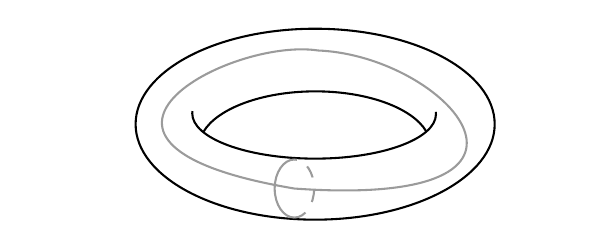
\begin{tikzpicture}[x=0.75pt,y=0.75pt,yscale=-1,xscale=1]
%uncomment if require: \path (0,300); %set diagram left start at 0, and has height of 300

%Shape: Ellipse [id:dp10888654123535657] 
\draw   (91,139) .. controls (91,113.59) and (129.73,93) .. (177.5,93) .. controls (225.27,93) and (264,113.59) .. (264,139) .. controls (264,164.41) and (225.27,185) .. (177.5,185) .. controls (129.73,185) and (91,164.41) .. (91,139) -- cycle ;
%Shape: Arc [id:dp9067895132467914] 
\draw  [draw opacity=0] (235.63,133.04) .. controls (235.69,133.42) and (235.71,133.81) .. (235.71,134.19) .. controls (235.67,146.12) and (209.35,155.7) .. (176.93,155.59) .. controls (144.5,155.48) and (118.25,145.73) .. (118.29,133.81) .. controls (118.29,133.42) and (118.32,133.05) .. (118.37,132.67) -- (177,134) -- cycle ; \draw   (235.63,133.04) .. controls (235.69,133.42) and (235.71,133.81) .. (235.71,134.19) .. controls (235.67,146.12) and (209.35,155.7) .. (176.93,155.59) .. controls (144.5,155.48) and (118.25,145.73) .. (118.29,133.81) .. controls (118.29,133.42) and (118.32,133.05) .. (118.37,132.67) ;
%Shape: Arc [id:dp7282595977083575] 
\draw  [draw opacity=0] (230.99,142.4) .. controls (224.37,131.23) and (202.8,123.1) .. (177.25,123.18) .. controls (151.77,123.27) and (130.31,131.5) .. (123.69,142.66) -- (177.34,149.79) -- cycle ; \draw   (230.99,142.4) .. controls (224.37,131.23) and (202.8,123.1) .. (177.25,123.18) .. controls (151.77,123.27) and (130.31,131.5) .. (123.69,142.66) ;

%Shape: Arc [id:dp4865327224674516] 
\draw  [draw opacity=0] (167.5,184) .. controls (167.5,184) and (167.5,184) .. (167.5,184) .. controls (162.25,184) and (158,177.73) .. (158,170) .. controls (158,162.27) and (162.25,156) .. (167.5,156) -- (167.5,170) -- cycle ; \draw  [color={rgb, 255:red, 155; green, 155; blue, 155 }  ,draw opacity=1 ] (167.5,184) .. controls (167.5,184) and (167.5,184) .. (167.5,184) .. controls (162.25,184) and (158,177.73) .. (158,170) .. controls (158,162.27) and (162.25,156) .. (167.5,156) ;
%Shape: Arc [id:dp049149640047466026] 
\draw  [draw opacity=0][dash pattern={on 4.5pt off 4.5pt}] (167.5,184) .. controls (167.5,184) and (167.5,184) .. (167.5,184) .. controls (172.75,184) and (177,177.73) .. (177,170) .. controls (177,162.27) and (172.75,156) .. (167.5,156) -- (167.5,170) -- cycle ; \draw  [color={rgb, 255:red, 155; green, 155; blue, 155 }  ,draw opacity=1 ][dash pattern={on 4.5pt off 4.5pt}] (167.5,184) .. controls (167.5,184) and (167.5,184) .. (167.5,184) .. controls (172.75,184) and (177,177.73) .. (177,170) .. controls (177,162.27) and (172.75,156) .. (167.5,156) ;

%Curve Lines [id:da7562826546508461] 
\draw [color={rgb, 255:red, 155; green, 155; blue, 155 }  ,draw opacity=1 ]   (179,103.5) .. controls (136.5,97) and (39.5,148.5) .. (167.5,170) .. controls (308,180) and (241,106) .. (179,103.5) -- cycle ;




\end{tikzpicture}
    }
    \caption{环面的拓扑性质}
\end{figure}

回忆一下,体系的希尔伯特空间维数为$2^{2N}$。当$2N-2$个边的自旋已经确定之后,系统的状态实际上已经确定了,因为约束条件\eqref{eq:toric-code-pair-condition}会确定剩下两条边的自旋。
换而言之,实际物理的希尔伯特空间维数只有$2^{2N-2}$。
这就意味着总希尔伯特空间$2^{2N}$分裂成了4支,或者说每个状态都有四重简并。
这个事实——环面上的Toric-code模型会出现基态四重简并——是\eqref{eq:toric-code-pair-condition}决定的,而\eqref{eq:toric-code-pair-condition}本身又来自环面的拓扑性质。
如果我们在哈密顿量中引入一个局部的扰动,基态能量和基态波函数显然会发生扰动,但是由于${A}$和${B}$的定义没有变化,系统拓扑没有变化,\eqref{eq:toric-code-pair-condition}也是始终成立的。
换句话说,环面上基态的四重简并是\concept{受到拓扑保护}的,局域的扰动不能让它消失。

用什么标记这四重简并?容易想到,完全可以定义一种全局性的闭弦算符,它贯穿整个环面,而由周期性边界条件它是闭弦算符。(这些算符的定义本身和拓扑紧密相关,显然如果系统被放在一个平面上那么根本没法定义全局性的闭弦算符)
分别沿着$x$轴和$y$轴定义
\begin{equation}
    {L}^x_\text{e} = \prod_{x} {\sigma}^z_{\vb*{i}}, \quad {L}^x_\text{m} = \prod_{x} {\sigma}^x_{\vb*{i}},
\end{equation}
并可以验证它们和哈密顿量是对易的,且它们构成一对对易稳定子。
这就意味着它们的本征值均为$\pm 1$,这就唯一地标记了四重简并。

以上两个弦算符标记的这种稳定的基态简并意味着Toric-code模型中显然有某种序,但这种序并不是使用对称性标记的,即和金斯堡-朗道理论中的那种局域的序是不同的。
的确,Toric-code中存在\concept{拓扑序}。

${L}^x_\text{e}$和${L}^x_\text{m}$将e粒子绕着$x$轴转动一圈,因此它们的本征值实际上给出了$x$方向类似于磁通量的一个通量,这个通量导致了一个Berry相位。

类似地还可以定义${L}^y_\text{e}$和${L}^y_\text{m}$,并且
\begin{equation}
    \acomm*{{L}^x_\text{e}}{{L}^y_\text{m}} = 0.
\end{equation}
我们知道
\begin{equation}
    \ket{0} = \ket{L_\text{e}^y=1, L_\text{m}^y=1},
\end{equation}
而使用这些关系可以证明,
\begin{equation}
    \begin{aligned}
        {L}^x_\text{e} \ket{0} &= \ket{L_\text{e}^y=1, L_\text{m}^y=-1}, \\
        {L}^x_\text{m} \ket{0} &= \ket{L_\text{e}^y=-1, L_\text{m}^y=1}, \\
        {L}^x_\text{m} {L}^x_\text{e} \ket{0} &= \ket{L_\text{e}^y=-1, L_\text{m}^y=-1}.
    \end{aligned}
\end{equation}
我们发现四重简并和四种基本的任意子正好能够对应上。这是拓扑序的一般特征:基态简并和任意子有对应,基态简并数目就是任意子数目的亏格次方。
我们这里是在亏格(洞的数目)为1的环面上工作,因此基态简并的数目为$4^1=4$种。
如果在亏格为0的球面上,基态简并的数目就是$4^0=1$种。
还有另一种方法也可以推导出这个结果。设亏格为$g$,由欧拉公式
\[
    V - E + F = 2 - 2g,
\]
于是
\[
    E - (V + F - 2) = 2g.
\]
而$V$是$A_s$格点的数目,$F$是$B_p$格点的数目,再减去\eqref{eq:toric-code-pair-condition}造成的两个约束,则$V+F-2$是一个二维表面Toric-code态的自由度个数。
Toric-code模型总的自由度个数为$E$,因此有$2g$个自由度用于标记简并态,由于每个自由度有两个取值,简并度为
\[
    2^{2g} = 4^g.
\]

我们看到,拓扑性质让基态简并出现,而基态简并意味着基态中可以有持续存在的弦——基态可以不是空无一物的!
这个看起来非常神奇——但是完全在预料之中——的性质让Toric-code模型成为一类允许出现弦网凝聚的模型中比较简单的一个。

\section{$\mathbb{Z}_2$规范理论}

Toric-code是一个严格可解模型;实际上,它的一些重要性质在哈密顿量形式更简单(但是不再严格可解)的所谓\concept{$\mathbb{Z}_2$规范理论}中也会体现出来。
历史上发生的事情其实是相反的:先有了$\mathbb{Z}_2$规范理论,然后再有了为了分析这一类的理论具有的性质而生造出来的Toric-code模型。

最广为人知的规范场论可能是电动力学,这是一个$U(1)$规范理论,其中电子场可以发生任意的局域相位转动,而与之配套的规范场——电磁场矢势——发生一个局域平移。
本文中我们不要$U(1)$这么大的对称性,而是只希望电子场或者不发生相位转动,或者相位就转动$\pi$,在这样的规范对称性——也就是\concept{\Ztwo规范对称性}下系统的动力学保持不变。
如果我们还是在通常的四维时空中工作那么局域\Ztwo变换就是不连续的:因为$0$和$\pi$不能连续过渡。
因此我们将在格点上工作,即研究格点规范场论。

\subsection{二维格子上的无物质场\Ztwo规范场理论}

\subsubsection{电子和\Ztwo规范场耦合}

在二维格子上,格点上的电子的动能项无非是从一个点跃迁到另外一个点,即
\begin{equation}
    {H}_0 = - \sum_{\vb*{i}, \vb*{j}, \alpha} t_{\vb*{i} \vb*{j}} {c}_{\vb*{i} \alpha}^\dagger {c}_{\vb*{j} \alpha}.
    \label{eq:hopping-hamiltonian}
\end{equation}
这个哈密顿量在局域\Ztwo变换下不是不变的。
现在假定出于某些原因,系统具有了\Ztwo规范对称性,那么为了加入局域\Ztwo对称性我们只能修改$t_{\vb*{i} \vb*{j}}$系数,使得它在\Ztwo变换下能够吸收掉电子场带来的变化。
容易看到,只需要指定
\[
    {c}_{\vb*{i} \alpha} \longrightarrow \eta_{i} {c}_{\vb*{i} \alpha}, \quad t_{\vb*{i} \vb*{j}} \longrightarrow \eta_i \eta_j t_{\vb*{i} \vb*{j}},
\]
就能够让哈密顿量具有局域\Ztwo对称性。由于$t_{\vb*{i} \vb*{j}}$只是在正负两种状态之间切换,可以引入一个规范联络$\sigma_{\vb*{i} \vb*{j}} = \pm 1$,于是用哈密顿量
\[
    {H} = - \sum_{\vb*{i}, \vb*{j}, \alpha} t_{\vb*{i} \vb*{j}} \sigma_{\vb*{i} \vb*{j}} {c}_{\vb*{i} \alpha}^\dagger {c}_{\vb*{j} \alpha}
\]
做路径积分,分别以${c}, {c}^\dagger$和$\sigma_{\vb*{i} \vb*{j}}$为积分变量即可得到一个\Ztwo规范理论。

现在我们回到正则量子化框架中,$\sigma_{\vb*{i} \vb*{j}}$在每一个格点引入了$\pm 1$两个状态,从而我们可以把它当成一个自旋$1/2$的自旋算符%
\footnote{实际上,这个“自旋算符”未必来自某个体系的内禀旋转不变性。
更加数学的说法是,由于每个格点都有两个状态,我们可以在每个格点引入一个$2\times 2$的厄米矩阵
\[
    {\sigma} = \pmqty{1 & 0 \\ 0 & -1}
\]
作为规范场对应的算符,而这正是泡利矩阵中的${\sigma}^z$。后面引入${\sigma}^x$等算符的目的也只是用于翻转规范场的状态。
}%
,从而哈密顿量为
\begin{equation}
    {H} = - \sum_{\vb*{i}, \vb*{j}, \alpha} t_{\vb*{i} \vb*{j}} {\sigma}^z_{\vb*{i} \vb*{j}} {c}_{\vb*{i} \alpha}^\dagger {c}_{\vb*{j} \alpha}
    \label{eq:minimal-z2-couple}
\end{equation}
希尔伯特空间为电子的态空间直积上每一点的自旋$1/2$空间。\Ztwo规范变换为
\begin{equation}
    {c}_{\vb*{i} \alpha} \longrightarrow \eta_{\vb*{i}} {c}_{\vb*{i} \alpha}, \quad {\sigma}_{\vb*{i} \vb*{j}}^z \longrightarrow \eta_{\vb*{i}} \eta_{\vb*{j}} {\sigma}_{\vb*{i} \vb*{j}}^z.
\end{equation}
特别的,如果\eqref{eq:hopping-hamiltonian}实际上是一个紧束缚模型,\eqref{eq:minimal-z2-couple}就成为
\begin{equation}
    {H} = - t \sum_{\pair{\vb*{i}, \vb*{j}}} {\sigma}^z_{\vb*{i} \vb*{j}} {c}_{\vb*{i} \alpha}^\dagger {c}_{\vb*{j} \alpha} + \text{h.c.}.
    \label{eq:tight-binding-z2}
\end{equation}
此时$\sigma_{\vb*{i} \vb*{j}}^z$实际上仅仅定义在格子的边上,即不需要对不相邻的点对$\pair{\vb*{i}, \vb*{j}}$也对应对应的$\sigma_{\vb*{i} \vb*{j}}^z$。

\subsubsection{\Ztwo规范场自身的哈密顿量}

将\eqref{eq:tight-binding-z2}中的电子自由度积掉%
\footnote{
    这当然要求电子是有能隙的,不过这其实没什么问题,如果\eqref{eq:tight-binding-z2}中的电子无能隙,我们就把它和一个普通的有能隙的紧束缚模型加起来再积掉电子即可。
    与电动力学相类比,积掉电子无非就是将介质中电子对电磁场的响应等效为介电常数和磁化率的修正。

    此外注意到,由于我们在正则量子化框架中工作,积掉电子自由度后希尔伯特空间缩小,原本的希尔伯特空间中的纯态将对应一个混合态。
    但是实际上这无关紧要,因为我们只需要假装不知道电子存在,分析\Ztwo规范场的态空间,最后计算配分函数即可,并不需要真的处理自旋系统的密度矩阵。}%
,得到仅仅关于\Ztwo规范场(而没有任何物质场)的一个低能有效理论。
严格做有关的计算是非常不现实的,但是无论如何,积掉电子自由度之后的哈密顿量本身肯定是\Ztwo规范不变的。我们首先先分析\Ztwo规范变换如何写成算符形式,然后分析积掉电子自由度之后的哈密顿量会是什么形式的。

电子自由度积掉之后规范变换就变成了
\begin{equation}
    {\sigma}_{\vb*{i} \vb*{j}}^z \longrightarrow \eta_{\vb*{i}} \eta_{\vb*{j}} {\sigma}_{\vb*{i} \vb*{j}}^z,
    \label{eq:pure-sigma-ztwo}
\end{equation}
也就是说对每一条边上的${\sigma}^z$本征态,规范变换或是不改变它,或是加一个负号。我们希望将\Ztwo规范变换写成算符的形式,为此注意到在自旋$1/2$中,算符${\sigma}^x$可以翻转${\sigma}^z$的本征态,且${\sigma}^x$是厄米算符,于是一条边上的规范场翻转就是
\[
    {\sigma}_{\vb*{i} \vb*{j}}^z \longrightarrow {\sigma}^x_{\vb*{i} \vb*{j}} {\sigma}_{\vb*{i} \vb*{j}}^z {\sigma}^x_{\vb*{i} \vb*{j}}.
\]
任何一个\Ztwo规范变换都可以拆解成一系列作用在格点上的规范变换相乘,而作用在格点$i$上的规范变换翻转和这个格点连接的四条边上的规范场,于是作用在格点$i$上的规范变换
\footnote{
    我们知道实际的系统都是定义在时空上的,所以似乎没有什么阻止我们在时间维上也做规范变换。
    这里的问题在于,\Ztwo规范场的路径积分形式需要离散化时间,处理起来非常不方便。以下我们将只考虑空间上的规范变换。
}%
为
\begin{equation}
    {Q}_i = \prod_{\pair{\vb*{i}, \vb*{j}}} {\sigma}^x_{\vb*{i} \vb*{j}} = \prod_{\pair{\vb*{j}, \vb*{i}} \in +_{\vb*{i}}} {\sigma}^x_{\vb*{i} \vb*{j}},
    \label{eq:z2-charge}
\end{equation}
于是规范不变量就是和所有${Q}_i$对易的算符。由于是低能有效理论,我们考虑最低阶的两个\Ztwo规范不变量,得到
\begin{equation}
    {H} = - K \sum_{\pair{\vb*{i}, \vb*{j}}} {\sigma}^x_{\vb*{i} \vb*{j}} - J \sum_{\Box} \prod_{l \in \Box} {\sigma}^z_{l}.
    \label{eq:z2-2d-hamiltonian}
\end{equation}
这就是只含有\Ztwo规范场的\emph{一个}有效理论(当然,实际上还有很多其它的\Ztwo规范理论,是取其它\Ztwo规范不变量得到的)。
关于为什么我们考虑了最低阶的两个\Ztwo规范不变量而不是别的(特别是,${\sigma}^x$是怎么被牵扯进来的),可以从两个角度考虑。
首先,最低阶的\Ztwo规范不变量具有最好的局域性,因此是更有可能出现的。
其次,在零温情况下我们此处给出的\Ztwo理论对应一个三维经典统计理论,这个三维经典统计理论当然也应该具有\Ztwo规范不变性。
我们知道这个三维经典统计理论的自由度实际上就是将\eqref{eq:z2-2d-hamiltonian}的自由度加上一个虚时间指标之后得到的结果,即$\{\sigma^z_{\vb*{i} \vb*{j}}(\tau)\}$。
由于没有$z$方向上的边上定义了$\sigma^z$自由度,我们可以直接沿用\eqref{eq:pure-sigma-ztwo}作为三维经典统计理论的\Ztwo规范变换。
三维经典统计理论的形式应该是
\[
    Z = \sum_{\sigma^z} \exp(\sum_{\tau} (J_{xy} \sum_{\Box} \prod_{l \in \Box} \sigma_l^z(\tau)  ) )
\]
% TODO

\subsubsection{去除规范自由度}

无论是\eqref{eq:tight-binding-z2}还是\eqref{eq:z2-2d-hamiltonian}都具有\Ztwo规范不变性,如果我们认为规范自由度不具有物理含义(它实际上有没有物理含义取决于我们关心的物理量是不是只涉及规范不变量),那么这两个哈密顿量就含有额外的自由度。
我们要设法把规范等价的构型全部映射到同一个构型上,而把规范不等价的构型映射到不同的构型上。
为此,我们将每个格子赋予一个格点坐标$I$,从而诸$\{i\}$和诸$\{I\}$形成对偶格点坐标。
设$\Box_I$为$I$号格子($I$标记了以所有的格子的中心为格点形成的新格子的格点坐标,称为\concept{对偶格子}),我们定义
\begin{equation}
    {\tau}^x_I = \prod_{l \in \Box_I} {\sigma}^z_l,
    \label{eq:def-tau}
\end{equation}
上标$x$看起来很奇怪,不过我们很快会发现其作用。这样\eqref{eq:z2-2d-hamiltonian}中的第二项就可以很容易地写出了。注意到$\tau^x_I$只有$\pm 1$两种取值,我们可以把它看成某个表象下的$x$方向泡利矩阵。
至于第一项,如果将${\sigma}_{\vb*{i} \vb*{j}}^x$作用在某个${\sigma}^z$表象下的基矢量上面,那么边$ij$上的$\sigma^z$反号,其余什么都不变,这就是说,设边$ij$由方格$I$和$J$共享,则由定义\eqref{eq:def-tau},$I$和$J$对应的$\tau^x$也反号,其余不变;
另一方面,将${\tau}^z_I {\tau}^z_J$作用在一个态上,则$I$和$J$对应的$\tau^x$均反号(同样依据泡利矩阵的性质,即$z$方向泡利矩阵可以翻转$x$方向泡利矩阵的本征态)。
两个算符的作用效果完全一样,所以实际上
\begin{equation}
    {\tau}^z_I {\tau}^z_J = {\sigma}^x_{\vb*{i} \vb*{j}},
\end{equation}
从而我们得到
\begin{equation}
    {H} = - K \sum_{\pair{I, J}} {\tau}^z_I {\tau}^z_J - J \sum_{I} {\tau}^x_I.
    \label{eq:z2-2d-tau-hamiltonian}
\end{equation}

现在没有规范冗余了——${\tau}^x_{I}$和${\tau}^z_I$都是规范不变量。
要看出自由度减少了多少,注意到二维格子中一个格子有四条边,每条边由两个格子分享,因此如果有$N$个格子(从而有$N$个格点),那么有$2N$条边。另一方面,只有$N$个方格。
因此如果只以${\tau}^z_I$为动力学自由度,则我们将希尔伯特空间的维数从$2^{2N}$降到了$2^N$。
丢自由度是正常的,因为在以上过程中我们抛弃了规范自由度,但是需要验证只以${\tau}^z_I$为动力学自由度是不是把一些并非规范自由度的自由度(它们没有出现在哈密顿量中)也抛弃了。
如果规范不等价的态给出不同的${\tau}^x_I$取值,我们就可以确定没有丢掉真正含有信息的自由度。
% TODO

在上述从$\sigma^z$到$\tau^x$的过程中我们丢失了一半的自由度,也就是说,有一半的$\sigma^z$自由度是可以随意指定的;指定这些$\sigma^z$自由度就是选取了一个规范。

\eqref{eq:z2-2d-tau-hamiltonian}正是横场伊辛模型,它是一个二维量子模型,其零温配分函数的精确形式对应一个三维经典统计模型,实际上这个三维经典统计模型就是一个各向异性的伊辛模型(在虚时间上的最近邻相互作用和空间方向上的最近邻相互作用不同)。
我们知道三维伊辛模型一定会出现相变,有一个顺磁相和一个铁磁相,这来自其普适类%
\footnote{
    虽然\eqref{eq:z2-2d-tau-hamiltonian}对应的经典统计模型是各向异性的,这并不改变其普适类,因为总是可以适当调节$\beta$的尺度让该经典统计模型变成各向同性的。
}%
,因此结论是,零温下横场伊辛模型——从而\Ztwo规范场——也会有一个相变,随着参数$K / J$的变化,从一个相切换到另一个相。

有一个看起来的佯谬:我们知道伊辛模型有一个全局\Ztwo对称性,可以将全部自旋翻转过来,得到一个不同的态,而与此同时哈密顿量保持不变。
实际上这个对称性在\Ztwo规范场中就是不存在的——等效的横场伊辛模型的相变破缺的就是这个对称性,由横场伊辛模型和\Ztwo规范场理论的等价性我们知道\Ztwo规范场理论也有一个相变,并且这个相变没有破缺任何对称性。
因此,在这里我们就已经知道了\Ztwo规范场有一个与对称性无关的相变了,它称为\concept{Ising*相变}。
和此相变有关的激发见\autoref{sec:z2-topo-excitation}。

\subsection{元激发和量子相变}

\subsubsection{规范荷和磁通量}

在$U(1)$规范场论中,设通过一个方格的磁通量为$\Phi$,则
\[
    \ee^{\ii \Phi} = \prod_{l \in \Box} t_{\vb*{i} \vb*{j}},
\]
于是在本文涉及的\Ztwo规范场中可以如法炮制地定义
\begin{equation}
    \ee^{\ii \Phi_I} = \prod_{l \in \Box_I} {\sigma}^z_{\vb*{i} \vb*{j}} = {\tau}^x_I,
\end{equation}
也即,我们用电子在格子上转一圈发生的相位改变来定义磁通量。与$U(1)$的情况不同,\Ztwo规范场中磁通量只有$0$和$\pi$两种,因为四个$\sigma^z$相乘要么是$1$要么是$-1$。
现在我们看到了${\tau}^x$的另一重意义:它标记了一个格子上的磁通量。
电磁场中的磁通量如果量子化的话需要一定条件,但是\Ztwo规范场中的磁通量就是量子化的,而且只有两个状态。
注意到$\tau_I^x$取$1$时能量较低而取$-1$时能量较高,我们可以将某个格子的磁通量取$\pi$当成一种激发态,称为\concept{m激发},以体现它和磁通量的相似之处。

另一个可以模仿电磁场引入的概念是\Ztwo规范荷,我们已经看到,\Ztwo规范变换对应的规范荷为\eqref{eq:z2-charge},这个量的取值只有$\pm 1$(因为是四个$\sigma^x$的乘积)。
由于\eqref{eq:z2-charge}守恒,我们有如下\Ztwo规范场的高斯定律:
\begin{equation}
    \prod_{j \in +} \sigma^x_{\vb*{i} \vb*{j}} = \text{\Ztwo -charge at $i$} = \const,
    \label{eq:gauss-z2}
\end{equation}
这个常数可以取$1$也可以取$-1$,但是不能一会是$1$,一会是$-1$。
这个额外的条件将希尔伯特空间划分成没有重叠的很多支,不同分支的\Ztwo规范荷分布不同。
虽然规范荷通常是通过规范场和物质场的耦合项引入的,在积掉物质场之后还是可以构造出规范荷的表达式,因为规范不变性的要求极大地限制了规范场荷物质场耦合的方式。
正如在电磁场中,即使我们积掉了物质场,麦克斯韦方程中还是会有一个电荷守恒方程
\[
    \pdv{\rho}{t} + \div{\vb*{j}} = 0
\]
一样——即使我们不知道电磁场实际上和一个物质场发生了耦合,我们还是可以将电荷当成电场线的某种特殊分布(源和汇),而以它们为某种激发。%
\footnote{
    \eqref{eq:gauss-z2}和麦克斯韦方程导出的电荷守恒方程有一个重要的区别,就是前者要求规范荷在每一点都守恒,而后者允许规范荷的流动。但这实际上并没有什么物理意义。
    麦克斯韦方程本身并不规定电荷应该如何流动(这是本构关系应该做的事情),因此,每一点的电荷密度算符和纯电磁场的哈密顿量也是对易的。
    在本节中尚未引入任何真的携带\Ztwo规范荷的场,如果引入了,本节中的${H}$就只是\Ztwo规范场的哈密顿量而不是完整的哈密顿量了,此时\eqref{eq:gauss-z2}的第一个等号当然仍然成立,但是每个点上的\Ztwo规范荷就未必总是不变的了,虽然规范对称性要求规范荷总量保持不变。 % TODO:总量是乘起来的还是加起来的??
    我们将这种没有动力学的规范荷称为\concept{测试规范荷},这个名称的意味是显然的;它相比有动力学的规范荷更容易处理,后者的哈密顿量在坐标表象下基本上不会是对角化的。

    还有一个表面上的不同是,麦克斯韦方程中显式地给出了电荷密度和电流密度,而此处的\Ztwo规范场理论中似乎没有。
    但这个其实只是记号的问题,电磁场的哈密顿量中实际上也没有出现电荷密度和电流密度。当我们从电磁场哈密顿量数学地导出运动方程时我们发现$\vb*{E}$的散度和$\vb*{B}$的旋度减去电场的时间导数似乎分别是某个东西的密度和流,从而暗示了“规范荷就在这里”,正如我们发现\Ztwo规范场中似乎有某个守恒荷\eqref{eq:z2-charge}一样。
}%
同理,在\Ztwo规范场中,$Q_i$取$-1$意味着更高的能量(计算一下能量期望值就知道),那么我们可以认为某个点$i$处$Q_i=-1$意味着这里出现了某个激发,从而一个\Ztwo规范荷被放置在了这里,无论其背后的机制是什么,无论是不是真的有一个物质场和\Ztwo规范场发生了耦合。%
\footnote{
    我们在\eqref{eq:tight-binding-z2}中是通过对电子的紧束缚模型引入局域\Ztwo规范对称性而得到一个\Ztwo规范理论的,但不难看出,我们这里引入的\Ztwo规范荷自由度肯定不是坐标表象下的电子激发,因为坐标表象下的电子激发的哈密顿量不是对角化的,或者直观地说电子会“四处乱跑”,而这里的\Ztwo规范荷只是测试规范荷。
}%
我们称这种激发为\concept{e激发},以体现它和电荷的相似性。

可以看到e激发和m激发的定义和Toric-code模型中的定义完全一样——实际上,这就是为什么Toric-code模型中的两种激发被命名为e激发和m激发。
相应的诸如弦算符、开弦、闭弦等的定义也和Toric-code模型中完全一样。

无物质场耦合的\Ztwo规范场中的e激发实际上是非常病态的一个东西,因为它没有任何涨落。我们可以把纯\Ztwo规范场中的e激发当成一个能隙无限大的元激发。
这里其实还有一个极限不能交换的问题:如果我们先让e激发的能隙趋于无穷大,然后计算配分函数,那么就得到了本节的纯\Ztwo规范场;但是如果我们先计算有物质场耦合的\Ztwo规范场模型的配分函数再让e激发的能隙趋于无穷大,那么 % TODO

我们尚未讨论定义e激发和m激发是否有意义。如果系统的低能自由度中实际上没有清晰可辨的这两种激发,那么引入这些概念毫无意义。
例如,可能存在这样的情况:e激发之间存在强烈的相互吸引,使得系统的低能自由度中根本没有长的开放的e弦,或者说,e激发被\emph{禁闭}了。
由于$J$和$K$能够调控e激发之间和m激发之间的相互作用,我们要问:在什么样的$J$和$K$取值范围中存在清晰可辨的e激发和m激发?

\subsubsection{自由相和禁闭相}

e激发和m激发禁闭的$J$和$K$取值和e激发和m激发解禁闭的$J$和$K$取值构成了两个量子相。
如果这两个量子相都是存在的,那么\Ztwo规范场应该存在一个量子相变。
根据\Ztwo规范场和横场伊辛模型的对偶关系,\Ztwo规范场的确有一个零温量子相变。
现在的问题是,\Ztwo规范场在零温下的两个相都是什么?

三维伊辛模型具有一个顺磁相和一个铁磁相,由于铁磁序的形成需要更多相互作用,$J/K$超过某个点时会出现顺磁相,否则出现铁磁相。
映射回二维横场伊辛模型,顺磁相意味着对偶格子上的各个$\tau$基本指向$x$方向,即有确定的磁通量;铁磁相意味着对偶格子上的各个$\tau$基本指向$z$方向,且要么几乎都为$1$要么几乎都为$-1$,没有确定的磁通量。
当$J$相对$K$很大时,系统处于顺磁相,此时的基态几乎就是每个$\sigma^z$都取$1$的态,此时直觉上看,费米子可以畅行无阻;而当$J$相对$K$很小时,系统处于铁磁相,此时的基态不是$\sigma^z$的本征态,投影在$\sigma^z$上有正有负,那么费米子似乎会被“迷惑”住(回忆一下,$\sigma^z$实际上是跃迁矩阵元),不知道怎么走。
那么,我们可以合乎情理地猜测,三维伊辛模型的顺磁相对应着\Ztwo规范场模型的一个解禁闭相,在其中e激发和m激发清晰可辨,而三维伊辛模型的铁磁相对应着\Ztwo规范场模型的一个禁闭相,在其中量子涨落破坏了e激发和m激发。

这样的论证当然是不够的,所以下面做一些半定量的论证。考虑\eqref{eq:z2-2d-hamiltonian}的格点路径积分(即虚时间轴也是离散化的),也即它对应的三维模型,定义
\begin{equation}
    W(C) = \expval{\prod_C \sigma^z_l(\tau)},
\end{equation}
其中期望值内部的算符乘积称为\concept{Wilson环算符}(如果它不闭合,那么就是弦算符),$C$是一个在虚时间方向上有延展的环路。
容易看出$W(C)$给出了从某个虚时间点开始产生一对e激发,按照$C$指示的轨迹扩散,经过一段时间之后又湮灭的概率(在经典理论中这是良定义的,因为没有任何不确定关系;具体有没有手段可以用量子测量的标准方法测出这个概率则是另外一回事),随着$C$扩大它理所当然会衰减,如果随着$C$扩大它衰减得很快那么就说明e激发总是成对地被束缚在一起。
我们本来可以使用两点格林函数来表征e激发被束缚的强度的,但是由于两点格林函数不是规范不变的,任何两点格林函数都是零。
$W(C)$的衰减方式有两种典型的形式:一种是\concept{面积定律},即
\begin{equation}
    W(C) \sim \ee^{-A},
\end{equation}
其中$A$是$C$围成的面积,另一种是\concept{周长定律},即
\begin{equation}
    W(C) \sim \ee^{-L}.
\end{equation}
设$C$持续时间为$\tau$,则按照虚时间演化,应该有
\[
    W(C) \sim \ee^{-\tau \Delta E},
\]
其中$\Delta E$是两个e激发同时出现造成的能量上升。我们马上可以看出,由于
\[
    A \sim \tau R,
\]
其中$R$是两个e激发的距离,如果面积定律成立,必然有
\[
    \Delta E \sim R,
\]
这是典型的禁闭效应:两个e激发离得越远,能量越高,当能量高到一定程度时涨落会导致新的e激发产生,从而产生两对离得非常近的e激发。
另一方面,如果周长定律成立,则
\[
    \Delta E \sim 1 + \frac{R}{\tau},
\]
而由于粒子通常不会跑太远,可以认为$\Delta E$基本上是一个常数,因此没有禁闭效应。

那么,前述横场伊辛模型给出的两个相是不是分别对应面积定律和周长定律?
我们尝试将$W(C)$映射到横场伊辛模型中,并在二维平面上计算$W(C)$。这实际上是有问题的,因为在用$W(C)$的行为判断是否有禁闭时,要求在时空上做Wilson回路,但此处我们单纯是在空间上做Wilson回路。
在\Ztwo规范场理论中这不会造成什么问题,因为它对应一个二维横场伊辛模型,后者对应一个三维经典伊辛模型,于是就有时间和空间的等价性。
由于Wilson回路能够使用的大部分模型都具有类似的性质,使用二维平面上计算出的Wilson回路来判断是否禁闭不会有问题,否则需要寻找别的回路算符。
因为$C$围成的区域内部的$\sigma^z$会被乘两次,于是就给出$1$,于是
\[
    \prod_{l \in C} \sigma^z_l = \prod_{l \in D} \sigma^z_l,
\]
依照$\tau^x$的定义即得到
\begin{equation}
    W(C) = \expval{\prod_{I \in D} \tau^x_I(\tau)},
\end{equation}
其中$D$是$C$围成的区域。
由于只有两个相,可以在$J/K$很小或很大时分别做微扰论,由此得到的关于相的结构的信息在整个相内部都是成立的。
$J \gg K$的情况对应顺磁相,系统基态形如
\[
    \ket*{\text{ground}} = \ket*{\tau^x = \rightarrow \rightarrow \cdots \rightarrow} + \frac{K}{J} \sum_{i, j} \ket*{\tau^x = \rightarrow \cdots \leftarrow_i \cdots \leftarrow_j \cdots \rightarrow} + \cdots,
\]
其中$i$和$j$相邻。
上式看起来很奇怪,不过真的去算期望会发现翻转两个$\tau^x$比翻转一个能量更低。(翻转相邻的两个${\tau}^x$的话,${\tau}^z_I {\tau}^z_J$项的期望不为零)
如果格点$i$和$j$在$C$内部,那么它不会对期望值有什么贡献,因为$-1$平方还是$1$;格点$i$和$j$在$C$外部那肯定也不会有什么贡献。
唯一会让期望值偏离$1$的激发是$i, j$中一个在$C$内部一个在$C$外部,于是我们有
\[
    \expval{\prod_{I \in D} {\tau}^x_I} \sim 1 - \frac{K}{J} L(C).
\]
那么,合理的猜测是,在顺磁相中应该有周长定律成立,于是没有禁闭。
铁磁相的讨论是类似的。 % TODO
我们仅仅讨论了两个极限情况,没有得到完整的$\ee$指数,但是一般的情况计算起来是非常困难的,此处略去。

总之,铁磁相($J / K \ll 1$)对应禁闭的\Ztwo模型的状态,其中e激发和m激发被禁闭;顺磁相则对应非禁闭的\Ztwo模型的状态。禁闭相中,e激发和m激发不再是有意义的低能自由度。
与通常的情况不同,在\Ztwo规范场模型中,顺磁相是非平凡的,铁磁相反而是平凡的。
由于禁闭相的基态非常接近${\tau}^z$的本征态,在其上讨论${\tau}^x$的排列模式——也就是m激发——并没有意义。
因此禁闭相中的“\Ztwo激发”——e激发和m激发——都没有意义,即在这里\Ztwo规范场的行为并不十分有趣。
当$J=0$时不可能出现很大的$J/K$,此时的二维\Ztwo规范场模型始终是禁闭的。
简单的计算可以证实这一点:$J=0$时
\[
    H = - K \sum_{\pair{\vb*{i}, \vb*{j}}} \sigma^x_{\vb*{i} \vb*{j}},
\]
现在设一条弦两端各有一个e激发,则弦上各点都有$\sigma^x = -1$,于是系统能量相比于基态能量的增量就是弦的长度乘以$K$。
因此会有一个全局不衰减的力将两个e激发拉在一起,即我们有一个禁闭相。
反之,在$K=0$时,m激发没有量子涨落,因此系统处在解禁闭相。
% TODO:这个胡扯的说法是哪里来的?当$J=0$时不可能出现很大的$J/K$,此时的二维\Ztwo规范场模型(称为\concept{Weigner模型})始终是禁闭的。

\subsubsection{Toric-code拓扑序}\label{sec:z2-topo-excitation}

有一点需要注意:虽然\eqref{eq:z2-2d-tau-hamiltonian}和\eqref{eq:z2-2d-hamiltonian}是对偶的,但在对称性、局域性等方面两者还是不一样的。就冗余性而言,\eqref{eq:z2-2d-hamiltonian}有\Ztwo规范对称性,但\eqref{eq:z2-2d-tau-hamiltonian}只有全局\Ztwo对称性;这两个模型实际上都是有冗余的,后者的冗余意味着什么我们马上可以看到。
同样,在\eqref{eq:z2-2d-hamiltonian}中显而易见的局域约束,在\eqref{eq:z2-2d-tau-hamiltonian}中也会以一种非常不平凡的形式呈现出来。

% 在\eqref{eq:z2-2d-hamiltonian}中只有${\sigma}^x$和${\sigma}^z$,如果我们假定规范场和外界的耦合项仅仅显含这两个算符,那么m激发就是成对出现的:容易证明
% \[
%    {\sigma}^z_i = {\tau}^x_I {\tau}^x_J,
% \]
%其中$i$是格子$I$和$J$共享的边,于是规范场和外界的耦合项只能够成对地产生和消灭m激发。m激发本身并没有禁闭(只需要在同一个格子的两条边上各作用一个${\sigma}^z$就能够创建一对不相连的m激发),但全局地看一定是成对的,从而全局地看,总磁通量一定是$0$。
% 只要\Ztwo规范场和外界通过${\sigma}^z$和${\sigma}^x$耦合,这就是一定成立的,也就是说这个性质——总磁通量为$0$,m激发成对产生——在任何局部的扰动下都是能够保持的。
% 需要注意的是如果我们将格点真的取为无限大,这个约束并没有意义,因此此时无法良定义一个总磁通量,或者直观地说,我们总是可以将成对的m激发的其中一个移动到无穷远,从而我们关心的区域中只有奇数个m激发。
% 在\eqref{eq:z2-2d-tau-hamiltonian}中m激发的个数是偶数(即$\tau^x$为$-1$的个数是偶数)完全不是显然的,因为“系统与外界的耦合通过${\sigma}^z$进行”在\eqref{eq:z2-2d-tau-hamiltonian}中无法简单地表示出来。

磁通量为$\pi$的m激发对应一个横场伊辛模型中的磁子(magnon)激发,由于它在\Ztwo规范场模型中的对应物是定义在顶点上的,也可以称它为\concept{vison激发}(Vortex-Ising-son,三个词根分别表示此类激发定义在格点上、和伊辛场有关、是元激发)。
横场伊辛模型中,$\tau^z \tau^z$项可以视为m激发的跃迁项,因为容易验证它可以让一个m激发跃迁到临近的格点上。

vison激发一定成对出现,通过分析\Ztwo规范场理论的希尔伯特空间可以直接确认这一点(我们在Toric-code模型中已经做过这件事了)。
表面上,与之对偶的横场伊辛模型\eqref{eq:z2-2d-tau-hamiltonian}可以有奇数个vison激发,因为可以将奇数个格子上的$\tau^x$设置为$-1$,但实际上这来自横场伊辛模型的全局\Ztwo冗余性。
将$K$调大,则$\tau^x$激发会越来越倾向出现,当出现得足够多时发生凝聚,此时就发生相变,从解禁闭相进入禁闭相。
因此\Ztwo规范场的解禁闭相中确实有一个序,这个序就体现在存在vison激发上,但是无法使用一个局域的序参量表示这个序。

两个vison或者说m激发可以看成一个开弦算符的两端,而系统中有有意义的开弦算符又意味着空间流形的非平凡拓扑性质可以被vison“看到”。

总之,实际上\Ztwo规范场的确有一个量子相变,然而这个量子相变和没有对称性任何关系:其有序相中特有的低能自由度是一些非局域的弦算符两端的任意子,而不是任何局域的序参量。
\Ztwo规范场理论\eqref{eq:z2-2d-hamiltonian}有零温量子相变,牵涉其中的两个相分别是任意子禁闭相和解禁闭相,解禁闭相中有拓扑序。
这个\Ztwo拓扑序称为\concept{Toric-code拓扑序},因为它和toric-code模型的拓扑序是一样的。

需要解释一下“一样的”是什么意思。
需要任意子动力学才能确定相变行为,正如通过金斯堡-朗道理论可以确定对称性自发破缺型相变的行为一样。
但是和金斯堡-朗道理论不同,知道了任意子表并不足以写出任意子的动力学。
因此,我们说“\eqref{eq:z2-2d-hamiltonian}中的拓扑序和Toric-code是一样的”似乎有失严谨,因为我们只说明了它们的任意子行为相同,没说明任意子的动力学一样。
但是通常我们不试图得到任意子的动力学,一方面因为这很困难,一方面因为没有必要——我们写出任意子只是为了描述\emph{解禁闭相}的\emph{普适}性质而暂时不关心相变时发生了什么又或者解禁闭相如何响应外加扰动。
与金斯堡-朗道理论相比较,金斯堡-朗道理论是可以描述相变时发生了什么的,而它描述有序相只需要一句话:“某某对称性被破缺了,低能自由度是某某序参量”。
在拓扑序中,怎么做出“某某对称性被破缺了”的有序相分类本身已经非常非平庸了,而通过它还不足以给出任意子的动力学。
对有能隙的\concept{阿贝尔拓扑序}(这就是说,拓扑序中两个任意子彼此交换后态矢量只是多出来一个相位),只需要任意子表就足够分类拓扑序:由于任意子激发态和基态之间有能隙,加入小的扰动并不会造成相变,从而,如果两个不同的模型均有有能隙的阿贝尔拓扑序,且有着同样的任意子表,那么可以缓慢地加入扰动,让两个模型的拓扑序长得完全一样而不造成相变,因此它们“本质上是相同的”。
与对称性驱动的相变做比较,阿贝尔的任意子表对应着对称性破缺后的相残余的对称性。
实际上也可以这样:两个任意子交换后得到的态矢量是一个矩阵乘以原来的态矢量,交换后的态矢量中可以有这两个任意子以外的任意子。这就是所谓的\concept{非阿贝尔拓扑序}。
对非阿贝尔的拓扑序,仅仅依靠任意子表是不够描述解禁闭相的,完整的描述需要使用一个范畴。

从横场伊辛模型\eqref{eq:z2-2d-tau-hamiltonian}中可以看到m激发是有能隙的,同样可以说明e激发也是有能隙的。
e激发和m激发可能有吸引相互作用,使得它们聚合形成的激发无能隙,不过当吸引相互作用强到了这种情况时单独讨论e激发和m激发又变得没有意义了(与电子类比,此时已经出现电子配对了)。
因此只讨论任意子表至少对\Ztwo规范场来说是合理的。

% 实际上,对$J=0$的二维\Ztwo规范场,通过适当选取规范还可以将它转化为一系列一维伊辛模型的组合。 
% 我们取规范

% 此时的禁闭相对应于顺磁相,因为伊辛模型中的${S}^z$就是磁通量。